% !TEX program = xelatex
% 编译：latexmk -xelatex main.tex
\documentclass[11pt]{ctexart}

\usepackage[a4paper,margin=2.5cm]{geometry}
\usepackage{graphicx}
\usepackage{amsmath}
\usepackage{booktabs}
\usepackage{array}
\usepackage{tikz}
\usetikzlibrary{arrows.meta,positioning,patterns,calc,backgrounds}
\usepackage{xcolor}
\usepackage[most]{tcolorbox}
\usepackage{caption}
\usepackage[colorlinks=true,linkcolor=blue!60!black,urlcolor=blue!60!black]{hyperref}
\usepackage{float}

\definecolor{plainC}{RGB}{235,244,255}
\definecolor{paperC}{RGB}{255,247,230}
\definecolor{numC}{RGB}{236,250,236}
\definecolor{warnC}{RGB}{255,236,236}

% —— 说人话框：给零基础读者的直觉解释 ——
\newtcolorbox{plainbox}[1][]{breakable,enhanced,colback=plainC,colframe=blue!45!black,
  title={\textbf{说人话} #1},fonttitle=\small,left=2mm,right=2mm,top=1mm,bottom=1mm}
% —— 论文依据框 ——
\newtcolorbox{paperbox}[1][]{breakable,enhanced,colback=paperC,colframe=orange!70!black,
  title={\textbf{论文依据} #1},fonttitle=\small,left=2mm,right=2mm,top=1mm,bottom=1mm}
% —— 关键数字框 ——
\newtcolorbox{numbox}[1][]{breakable,enhanced,colback=numC,colframe=green!40!black,
  title={\textbf{关键数字} #1},fonttitle=\small,left=2mm,right=2mm,top=1mm,bottom=1mm}
% —— 踩坑记录框 ——
\newtcolorbox{warnbox}[1][]{breakable,enhanced,colback=warnC,colframe=red!60!black,
  title={\textbf{踩过的坑} #1},fonttitle=\small,left=2mm,right=2mm,top=1mm,bottom=1mm}

\setlength{\parskip}{0.45em}

\title{\textbf{从``逐点分类''到``一栋一栋的楼''}\\[0.3em]
\Large 建筑单体分割与噪声清除（管线步骤 2--3）零基础讲义}
\author{Columbus LiDAR $\to$ LOD2 管线 · 汇报准备材料}
\date{2026 年 8 月 30 日}

\begin{document}
\maketitle

\begin{plainbox}[：这本讲义讲什么]
上一步（RandLA-Net 语义分割）只回答了``\textbf{这个点是不是建筑}''；本步要回答
``\textbf{这个点属于哪一栋楼}''，并把混进来的``假建筑''（桥、匝道、树冠、电线）清理出去。
讲义假设你没有任何点云、图像处理或机器学习背景，每个术语第一次出现时都会解释；
读完后你应当能向导师完整讲出：用了哪篇论文的什么方法、每一步为什么这么设计、
以及 2{,}296 $\to$ 2{,}267 每一个数字的来龙去脉。
\end{plainbox}

\tableofcontents
\newpage

\section{模块 1 · 任务与起点：上一步交给我们什么，这一步要做出什么}

\subsection{我们手里的数据长什么样}

整个项目的原始数据是\textbf{机载激光雷达（LiDAR）点云}。它的获取方式一句话就能说清：
飞机沿着测区上空飞行，向地面连续发射激光脉冲，测量每束激光打到物体反射回来的时间，
从而算出打中位置的三维坐标。每束激光的落点就是一个``点''，
千万个点合在一起就是``点云''——可以想象成\textbf{给整个城市拍了一张由无数小点组成的三维照片}：
屋顶上有点、地面上有点、树冠上也有点。

每个点至少带三个数：$x$（东西向位置）、$y$（南北向位置）、$z$（高度——注意它是
相对统一高度基准面测的，测绘上叫``高程''，不是``离地面多高''）。
本项目数据的坐标单位是\textbf{美制测量英尺}（ftUS，1 ftUS $\approx$ 0.3048 米，
这是美国政府测绘数据的惯例单位）；我们在计算时统一换算成米。

\begin{numbox}[：本项目的原始数据]
研究区为哥伦布市近东区约 2.76 平方公里的住宅区；
数据来自 USGS（美国地质调查局）2019 年航飞，共 19 块瓦片（tile，即数据分块文件），
合计 \textbf{76{,}351{,}005 个点}，平均密度约 \textbf{30 点/平方米}
——如果把点想象成均匀铺开，相邻点相距约 18 厘米
（实际分布并不均匀，这只是个数量级的直觉）。
\end{numbox}

\subsection{上一步（RandLA-Net）已经做了什么：语义分割}

原始点云只有坐标，没有``身份''：计算机不知道哪个点是屋顶、哪个点是树。
我们的整套处理流程（下文简称\textbf{管线}，pipeline，一步接一步的加工流水线）第 1 步
用一个叫 RandLA-Net 的\textbf{深度学习网络}（一类从人工标注的示例中自动学出判断规律的程序）
做了\textbf{语义分割}（semantic segmentation）——直白地说，就是\textbf{给每一个点贴一张类别标签}。
本项目用四类标签（编号沿用美国摄影测量与遥感学会 ASPRS 制定的行业标准类别码）：

\begin{center}
\begin{tabular}{cll}
\toprule
类别码 & 含义 & 占比 \\
\midrule
2 & 地面（马路、草坪、裸土） & —— \\
5 & 植被（树冠、灌木） & —— \\
6 & \textbf{建筑（屋顶、部分墙面）} & 约 863 万点，占全部点的 11.3\% \\
1 & 其他（车辆、电线等零散物） & —— \\
\bottomrule
\end{tabular}
\end{center}

于是我们得到了 19 块``每个点都带类别标签''的点云。本讲义的一切都从这份结果出发：
\textbf{把标签为 6 的约 863 万个点拿出来加工}。下文把它们简称``建筑点''，
但请记住：这只是模型打的标签，里面混着被错标的桥、树冠、电线
——清理它们正是步骤 3 的任务。另外两类标签也有用：标签 2（地面）在第 3 步会用到
（用来算``离地高度''），标签 5（植被）在后面的追溯修正中用来抓混进来的树冠。

\subsection{本步的任务：从``语义''到``实例''}

语义分割只回答``是什么''，不回答``是哪一个''。全区两千多栋楼的屋顶点，标签全都是 6，
彼此之间没有任何区分。而后续的屋顶重建必须\textbf{一栋一栋地做}
（每栋楼单独提取屋顶平面、单独拼模型），所以必须先把建筑点\textbf{按栋分开}
——这一步叫\textbf{实例分割}（instance segmentation），行业里也叫\textbf{建筑单体化}。
``实例''就是``具体的一个个体''：同样是``建筑''这个类别，1 号楼和 2 号楼是两个不同的实例。

\begin{figure}[H]
\centering
\begin{tikzpicture}[scale=0.82, every node/.style={font=\small}]
% ---- 左：语义分割 ----
\begin{scope}
\node[font=\bf\small] at (2.6,3.1) {语义分割的结果（第 1 步）};
\fill[blue!30] (0,0) rectangle (1.5,1.2);
\fill[blue!30] (2.0,0.1) rectangle (3.4,1.4);
\fill[blue!30] (3.9,0) rectangle (5.2,1.1);
\node at (0.75,0.6) {建筑};
\node at (2.7,0.75) {建筑};
\node at (4.55,0.55) {建筑};
\node[text width=5.2cm, align=center] at (2.6,-0.8)
  {三栋楼颜色相同：只知道``都是建筑''\\ 分不清彼此};
\end{scope}
% ---- 右：实例分割 ----
\begin{scope}[xshift=7.3cm]
\node[font=\bf\small] at (2.6,3.1) {实例分割的目标（本步）};
\fill[red!40] (0,0) rectangle (1.5,1.2);
\fill[green!45] (2.0,0.1) rectangle (3.4,1.4);
\fill[orange!55] (3.9,0) rectangle (5.2,1.1);
\node at (0.75,0.6) {1 号楼};
\node at (2.7,0.75) {2 号楼};
\node at (4.55,0.55) {3 号楼};
\node[text width=5.2cm, align=center] at (2.6,-0.8)
  {每栋楼一个编号（instance\_id）\\ 楼内所有点共享这个编号};
\end{scope}
\end{tikzpicture}
\caption{语义分割 vs.\ 实例分割：本步的任务就是从左图走到右图。}
\label{fig:sem-vs-inst}
\end{figure}

本步做完后，每个建筑点会多带一个整数编号 \texttt{instance\_id}：
同一栋楼的点编号相同，不同楼编号不同。后续所有步骤（屋顶平面提取、模型装配、精度评价）
都以这个编号为``楼''的定义。

\subsection{为什么这件事不是``顺手就能做''的}

直觉上似乎很简单：``挨在一起的点算一栋楼''。但真实数据里有两类拦路虎，
分别对应本步的两个子任务：

\textbf{拦路虎一：楼和楼``粘''在一起（对应步骤 2：单体分割）。}
本区是独栋住宅区，相邻两栋楼之间的侧院间隙常常只有 1.5--2.5 米。
点云是离散的、屋檐还会向外挑出，两栋楼的点在空间上非常接近。
而计算机做分组时，总要先定一个``多近才算连在一起''的尺度：尺度设小了，
一栋楼自己会碎成几块；设大了，隔着窄侧院的两栋楼就被当成一体。
一旦这个尺度处理不当（后面会看到 v1 版本的真实教训），整排房子会被连成``一栋''，
这种错误叫\textbf{欠分割}（under-segmentation，该分开的没分开）。
反过来，一栋楼如果被拆成好几块，叫\textbf{过分割}（over-segmentation）。
单体分割的全部功夫，就是在这两种错误之间走钢丝。

\textbf{拦路虎二：混进来的``假建筑''（对应步骤 3：噪声清除）。}
RandLA-Net 不是完美的，它会把一些``长得像建筑''的东西错标成类别 6：
高架桥面、立交匝道、成排的树冠、电力线。这些东西如果不清理，
会一路混到最后变成一个个``假房子模型''。而且越到后面越难发现
——桥面本身就是一块平整的板，后续算法用数学平面去近似它时，比近似真屋顶还顺利，
根本不会报错。所以必须\textbf{在程序开始逐栋重建之前、以``栋''为单位}把它们拦下来，
这道关卡我们称为 Gate A（gate＝闸门，A 表示它是全管线的第一道质量闸）。

\begin{plainbox}[：一个比喻串起两个子任务]
把 863 万个``被标成建筑''的点想象成一大袋混在一起的乐高零件。步骤 2 是\textbf{分拣}：
按空间位置把零件分成 2{,}296 小袋，每袋暂时当作``一栋候选建筑''；步骤 3 是\textbf{质检}：
逐袋检查，把``根本不是楼''的袋子（桥、树、电线）整袋挑出去。
最后剩下 2{,}267 袋通过质检的候选建筑，交给下一步拼屋顶。目标是``一袋恰好一栋楼''
——至于做到了几分，靠人工抽查与最终的精度评价来回答，而不是靠这个数字本身。
（2{,}296 与 2{,}267 怎么来的，模块 4--6 会逐项对账。）
\end{plainbox}

\subsection{本步在整条管线中的位置}

\begin{center}
\begin{tikzpicture}[node distance=0.55cm, every node/.style={font=\small}]
\tikzstyle{stage}=[draw, rounded corners, minimum height=0.9cm, text width=2.5cm, align=center]
\tikzstyle{cur}=[stage, fill=blue!15, draw=blue!60!black, thick]
\node[stage] (s1) {第 1 步\\ 语义分割};
\node[cur, right=of s1] (s23) {\textbf{第 2--3 步}\\ \textbf{单体化+清噪}};
\node[stage, right=of s23] (s45) {第 4--6 步\\ 屋顶平面·线索·轮廓};
\node[stage, right=of s45] (s7) {第 7 步起\\ 模型装配$\cdots$};
\draw[-{Stealth}] (s1) -- (s23);
\draw[-{Stealth}] (s23) -- (s45);
\draw[-{Stealth}] (s45) -- (s7);
\end{tikzpicture}
\end{center}

输入：19 块带语义标签的点云（\texttt{01\_semantic\_randlanet/results/preds/}）；
输出：一份带 \texttt{instance\_id} 的干净建筑点云文件 \texttt{buildings\_clean.laz}
（\texttt{.laz} 是点云的压缩文件格式；文件存放在 \texttt{02\_03\_instance\_seg/output\_v2/}），
外加一张逐实例的``审计表''（记录每个实例的属性和去留原因，模块 5--6 详述）。

\begin{plainbox}[：模块 1 小结]
\begin{itemize}
\item 起点：约 7{,}635 万点的点云，每点已带类别标签；其中被标为建筑的约 863 万个（11.3\%）。
\item 任务：给建筑点按栋编号（实例分割），并剔除``假建筑''（Gate A 质检）。
\item 两大风险：欠分割（楼粘成一条）与假建筑混入（桥/树/电线）；
      下面两个模块先讲我们参考了谁的方法、为什么这么选。
\end{itemize}
\end{plainbox}

\newpage
\section{模块 2 · 参考论文与技术路线：站在谁的肩膀上，为什么这么选}

做汇报时导师一定会问：``这方法是你发明的，还是参考了谁？''本模块把答案一次说清。
先给结论：\textbf{总体路线参考 Song \& Jung 的``栅格化 + 图像形态学''无监督工作流，
拆楼粘连用 Beucher \& Meyer (1993) 的经典分水岭算法，噪声清除的关键约定取自
荷兰 3D BAG 生产线（Peters et al.\ 2022）}；在此骨架上我们针对本区数据做了三处自己的改造
（不做闭运算、以高度面做分水岭地形、非对称碎片吸收——模块 3--4 详解）。

\subsection{选方法前先明确判断标准}

模块 1 说了本步的两个子任务（按栋分开、剔除假建筑）。挑方法时我们定了三条标准：

\begin{enumerate}
\item \textbf{可解释、可审计}：每个决定（这两栋为什么分开？那个实例为什么被删？）
      都要能指着中间产物讲清楚——这是本项目的验收习惯（每一步都在 CloudCompare
      里人工抽查，CloudCompare 是一款免费的点云查看软件）。
\item \textbf{不依赖额外训练数据}：语义分割已经花掉了标注预算，单体化最好``拿来就能用''。
\item \textbf{适配本区场景}：独栋住宅为主、楼间距小（1.5--2.5 米）、树多遮挡重。
\end{enumerate}

第 3 条不是一句空话，三个场景特点在方案里各有对应的招数：
楼间距小 $\to$ 分水岭按高度谷拆粘连（模块 4）；树冠被误标成建筑 $\to$
Gate A 与追溯修正逐实例清除（模块 5--6）；树遮挡造成屋顶空洞 $\to$
逐块补洞机制（模块 3）。当然它们各有局限，讲到时逐一说明。

\subsection{一个先决选择：要不要用官方``建筑底图''（footprint）}

在讲具体算法之前，有一个更根本的路线分岔。\textbf{footprint（建筑底图/轮廓）}
指政府地籍或测绘部门维护的每栋建筑的平面轮廓多边形——相当于官方已经画好的``每栋楼的地界''。

\begin{paperbox}[：两条路线]
\textbf{footprint-guided（有底图路线）}：把现成轮廓当输入，点云只负责``往轮廓里填高度''。
单体化问题被底图直接解决——一个轮廓就是一栋楼。这是\textbf{大型生产项目的常见路线}：
荷兰 3D BAG 项目以官方地籍轮廓 + LiDAR 重建了全国约 1{,}000 万栋建筑
（Peters, R.\ et al.\ 2022, \textit{PE\&RS} 88(3)。LoD2 指``带屋顶形状的三维建筑模型''
这一细节等级，是本管线的最终目标产品）；格拉斯哥的 LoD2 模型
（覆盖约 100 km\textsuperscript{2} 核心区，全域另有更粗的 LoD1）
也走有底图路线——值得注意的是，它的底图并非官方地籍，而是\textbf{从点云栅格掩膜
提取再正则化得到的轮廓}，配合开源重建工具 City3D（Huang et al.\ 2022）的
有底图模式使用。思想源头可追到 Vosselman \& Dijkman (2001) 用地面图辅助重建的经典工作。

\textbf{footprint-free（无底图路线）}：只用点云自己解决单体化——就是本项目的选择。
\end{paperbox}

为什么放着这条``省事的常见路线''不用？三个理由：
（a）\textbf{研究目标}本身就是检验``纯点云能走多远''——很多地区没有高质量底图，
方法要有普适性；
（b）官方底图有时效问题（新建、翻建、拆除不同步）；
（c）最重要的一条：本县（Franklin County）其实\textbf{有}官方 footprint，
但我们故意不让它进管线，而是留作最后第 9 步的\textbf{精度评价基准}
——同一份数据既当输入又当考卷，考试就没有意义了。

\subsection{主参考：Song \& Jung 的``栅格化 + 形态学''工作流}

\begin{paperbox}[：主参考文献]
Song, H., Jung, J.\ An Unsupervised, Open-Source Workflow for 2D and 3D
Building Mapping From Airborne LiDAR Data. \textit{IEEE JSTARS} 17
（2024 年正式收卷，2023 年在线发表；IEEE JSTARS 是美国电气电子工程师学会的
应用地球观测与遥感专题期刊）。
\end{paperbox}

这篇论文的核心思想只有一句话：\textbf{把三维点云``拍扁''成二维格子图，
然后用图像处理里成熟的工具来切建筑图斑}。``栅格化''``形态学''这些词模块 3 会从零讲；
这里先说清\textbf{为什么选它当骨架}：

\begin{enumerate}
\item \textbf{无监督}：整个流程不需要任何训练样本，拿到分类点云直接跑——满足标准 2。
\item \textbf{每一步都看得见}：中间产物是一张张图像，哪一步出错一眼可见——满足标准 1。
      后面会看到，我们正是靠``把中间图像画出来给用户检查''抓住了 v1 的大错误。
\item \textbf{计算便宜}：863 万个三维点的问题被压缩成一张几千$\times$几千的二维图像，
      个人电脑即可完成全区处理，无需服务器或显卡。
\item \textbf{天然衔接}：需要说明，原论文是从\textbf{原始} LiDAR 做起的完整工作流
      （含地面提取、建筑与树木的区分等环节）；我们\textbf{只借用其中
      ``栅格化 + 图像形态学制图''这一段}，并把自己第 1 步得到的建筑点作为这一段的输入
      ——相当于用深度学习语义分割替换了它的前半程，两者接口恰好吻合。
\end{enumerate}

要诚实说明的差别：Song \& Jung 的目标是\textbf{制图}（在地图上画出建筑图斑），
我们的目标是\textbf{实例}（每栋楼一个编号、还要把编号写回每一个三维点）。
所以我们沿用它``栅格化 + 形态学 + 连通域''的骨架，但在两处走得更远：
粘连楼的拆分（模块 4 的分水岭）和标签回写到点（模块 3 末尾）。

\subsection{拆粘连的关键工具：分水岭算法}

\begin{paperbox}[：经典算法文献]
Beucher, S., Meyer, F.\ (1993). The morphological approach to segmentation:
the watershed transformation. 收录于 \textit{Mathematical Morphology in Image
Processing}。——图像分割领域最经典的算法之一，30 多年来是``分开粘连目标''的标准工具
（显微镜下粘连的细胞、粘在一起的硬币，都是它的经典应用场景）。
\end{paperbox}

一句话直觉（模块 4 用图详细讲）：把图像看成\textbf{地形}，往里``灌水''，
水从不同的洼地涨起来，两片水相遇的地方\textbf{筑坝}——坝就是分割边界。
我们用它的\textbf{marker 控制版本}（marker-controlled watershed）：
先指定``水从哪几个源头涨起''，拆出来的块数就由源头数量控制，
噪声洼地不再各自成块——经典分水岭``一个噪声就多一块''的过分割毛病被压住了。
当然，责任随之转移到``源头找得准不准''上：找多了照样过分割、找少了照样欠分割，
所以模块 4 里``源头''的产生自带面积门槛把关。

\subsection{没有选的路线，以及为什么（导师大概率会追问）}

\textbf{（a）纯``连通域''为什么不够？}连通域（挨着的算一块，模块 3 详讲）
是最朴素的单体化。Yang et al.\ (2022, \textit{Int.\ J.\ Remote Sensing})
指出了这类做法的困难区间：\textbf{当楼间距逼近点间距时，简单的邻近分组容易失败、
相邻建筑难以分开}（他们因此提出``先把点组成小对象、再用对象间关系图合并成建筑''
的实例分割方法）。本区的账要算细一点：侧院 1.5--2.5 米、格距 0.5 米，
直接相除是 3--5 个格子宽的空隙；但屋檐每侧向外挑出 0.3--0.6 米，
两侧合计再吃掉 1--2 格，实际留在图上的空隙常常只有 2--4 格。
空隙本身不会让连通域出错——真正把空格``填上''的是三种东西：
落在缝里的零星误标点、伸进缝里的树冠、以及（v1 教训里的）闭运算。
缝越窄，越容易被填死——所以连通域只能当第一刀，粘连要靠分水岭补刀。

\textbf{（b）为什么不用更新的深度学习 / 图聚类实例分割？}同问题较新的代表工作之一是
Li, J.\ et al.\ (2026)：City-scale building instance segmentation via
structure-aware method（\textit{Int.\ J.\ Applied Earth Observation and
Geoinformation} 146:105086）。该文包含语义分割网络、新数据集等多项内容，
与我们对应的是其中的 \textbf{SI-DVDC 实例聚类}部分，思路是``密度可达的图聚类''：
把点（或小块）当作\textbf{节点}，空间上接近的节点之间连线，构成一张``图''
（网络结构意义上的图，不是图片）；能沿着足够密集的连线互相走到的节点，归为同一栋楼。
不选它当主线的理由：其一，它的强项是大城市复杂粘连建筑群，本区以独栋住宅为主，
用不上这份复杂度；其二，图聚类的中间状态难以像图像那样逐步画出来给人检查，
不符合我们``每步可审计''的工作方式；其三，引入新方法有调参与复现成本。
它被记为\textbf{候选兜底方案}（我们并未实际运行它，因此不称``对照''）
——如果形态学路线在某类场景失效，这是首选替代项。

\subsection{路线总览}

\begin{center}
\small
\begin{tabular}{p{3.1cm}p{3.6cm}p{3.9cm}p{3.6cm}}
\toprule
子问题 & 选用方法 & 依据文献 & 我们的改造 \\
\midrule
点云 $\to$ 可处理的图 & 0.5 m 占据栅格 & Song \& Jung 2024 & 每格 $\geq$2 点才算占据；\textbf{不做闭运算}（v1 教训，模块 3） \\
初步分块 & 8-连通域 & Song \& Jung 2024；困难区间见 Yang 2022 & 逐块补内部空洞（不向外桥接） \\
拆开粘连的楼 & marker 分水岭 & Beucher \& Meyer 1993 & 用 $-z_{\max}$ 高度面当地形；腐蚀取核当 marker（模块 4） \\
防过分割 & 碎片吸收 & —— （工程设计） & \textbf{非对称}规则：只许小并大（模块 4） \\
假建筑清除 & 离地高度 + 形状规则 + 人工判读 & 地面高度取``周边 4 m 内地面点第 5 百分位''借自 3D BAG（Peters 2022）；``桥必须在实例级清除''的机理见模块 5 & 3D BAG 依赖官方轮廓定``周边''，我们改用实例自身外扩 4 m 环；规则只``捞候选''，删除一律人工判读 + 原因码存档（模块 5） \\
候选兜底 & 图聚类实例分割 & Li et al.\ 2026 (SI-DVDC 部分) & 未运行，保留为替代路线 \\
\bottomrule
\end{tabular}
\end{center}

\begin{plainbox}[：模块 2 小结（汇报口径）]
一句话向导师交代：``我们走 footprint-free 路线（官方底图留作考卷），
主体沿用 Song \& Jung 的无监督栅格化工作流，粘连用经典 marker 分水岭拆分，
清噪沿用 3D BAG 生产线的离地高度约定；在闭运算、分水岭地形与碎片吸收三处
做了针对本区数据的改造，改造依据是 v1 版本的实测失败教训。''
\end{plainbox}

\newpage
\section{模块 3 · 步骤 2 上篇：把点云变成``图上的楼块''}

从这个模块起讲具体算法。步骤 2（单体分割）在代码里是一条流水线
（\texttt{instance\_segmentation\_v2.py}），本模块讲前半段：
\textbf{栅格化 $\to$ 连通域}，以及一个用真实失败换来的设计决定（\textbf{不做闭运算}）。
后半段（拆粘连、防过分割）在模块 4。

\subsection{第一刀：把三维点云``拍扁''成二维格子图（栅格化）}

\textbf{栅格化（rasterization）}就是把连续空间切成规则小方格（想象一张方格纸铺在地图上），
再统计每个格子里落了什么。我们在俯视视角下铺一张\textbf{边长 0.5 米}的方格纸，
把 863 万个建筑点按 $(x,y)$ 坐标投进格子里。

为什么可以放心``拍扁''（丢掉俯视重叠信息）？因为在住宅区里，
两栋不同的楼在俯视图上不会上下重叠——``按栋分开''本质上是个二维问题。
但注意：我们并没有真的丢掉高度。每个格子除了记``落了几个点''，
还记下了\textbf{格内最高点的高程 $z_{\max}$}——这张``高度图''在模块 4 的分水岭里是主角。

接着定义哪些格子``算数''：

\begin{center}
\fbox{\parbox{0.9\textwidth}{\centering
\textbf{占据规则}：一个格子里落入 $\geq 2$ 个建筑点，才算``被建筑占据''。
}}
\end{center}

为什么是 $\geq 2$ 而不是 $\geq 1$？这是\textbf{第一道防线}：RandLA-Net 偶尔会把一两个零星的
树点、车点错标成``建筑''。若 1 个点就算占据，一串零星错点就能在两栋楼之间搭出一条
``一点宽的桥''，把两栋楼连起来。要求每格至少 2 点，孤立错点自动失效。
说它是``第一道''防线是有分寸的：它只压低搭桥的概率，不能保证根除
（理论上两个错点挤进同一格仍能过关）——彻底的保障靠的是它与后续机制的叠加
（模块 4 的分水岭还会按高度把粘连切开）。代价方面：全区平均密度约 30 点/m\textsuperscript{2}
（0.5 m 格子平均 7--8 个点），完整屋面的格子远超 2 点的门槛；
真正可能受损的是屋顶边缘和被树遮挡处的稀疏格子——这些格子里的点先被放下，
模块 4 结尾有专门的``孤儿点回挂''机制把它们捡回来。

\begin{figure}[H]
\centering
\begin{tikzpicture}[scale=0.62]
% 网格
\draw[step=1, gray!40, thin] (0,0) grid (10,5);
% 房子1的点（左）
\foreach \p in {(0.3,1.2),(0.7,1.5),(1.2,1.3),(1.5,1.8),(0.5,2.3),(1.3,2.6),(1.7,2.2),(2.3,1.4),(2.6,1.7),(2.2,2.5),(2.7,2.3),(0.4,3.3),(1.4,3.5),(2.5,3.4),(1.9,3.2),(0.8,2.7),(2.8,3.7),(1.1,1.9),(2.1,1.9),(0.6,3.6)}
  \fill[blue!70] \p circle (2.2pt);
% 房子2的点（右）
\foreach \p in {(6.4,1.3),(6.8,1.6),(7.3,1.4),(7.6,1.9),(6.6,2.4),(7.4,2.7),(7.8,2.3),(8.4,1.5),(8.7,1.8),(8.3,2.6),(8.8,2.4),(6.5,3.4),(6.2,3.7),(7.5,3.6),(7.8,3.3),(8.6,3.5),(8.0,3.3),(6.9,2.8),(7.2,2.0),(8.2,2.0),(6.3,2.9),(8.9,3.1)}
  \fill[blue!70] \p circle (2.2pt);
% 中间一个零星错点
\fill[red!80] (4.6,2.4) circle (2.6pt);
\node[red!80, font=\scriptsize] at (4.6,3.0) {零星错点（1 点）};
% 占据格着色
\begin{scope}[on background layer]
\foreach \c in {(0,1),(1,1),(2,1),(0,2),(1,2),(2,2),(0,3),(1,3),(2,3)}
  \fill[blue!15] \c rectangle +(1,1);
\foreach \c in {(6,1),(7,1),(8,1),(6,2),(7,2),(8,2),(6,3),(7,3),(8,3)}
  \fill[blue!15] \c rectangle +(1,1);
\end{scope}
\node[font=\small] at (1.5,-0.6) {楼 A：格内点多 $\Rightarrow$ 占据};
\node[font=\small] at (7.5,-0.6) {楼 B：占据};
\node[font=\small, red!70!black] at (4.5,0.4) {仅 1 点的格子不算占据};
\end{tikzpicture}
\caption{栅格化与占据规则：点（蓝）投进 0.5 m 格子；$\geq2$ 点的格子（浅蓝）构成``占据图''；
孤立错点（红）无法形成占据格，从源头掐断``一点桥''。}
\label{fig:raster}
\end{figure}

这一步结束，863 万个建筑点的问题被压缩成一张黑白图像：黑格 = 有建筑，白格 = 没有。
后面的所有操作都在这张图上做，这正是模块 2 说的 Song \& Jung 路线的精髓
——\textbf{图像化之后，几十年积累的图像处理工具全部可用}。

\subsection{第二刀：连通域标记——``挨着的格子算同一块''}

\textbf{连通域（connected component）}是图像处理最基础的概念：
在黑白图上，把互相挨着的黑格归成一``块''，每块发一个编号。
``挨着''有两种定义：\textbf{4-连通}只认上下左右四个邻居；
\textbf{8-连通}把四个斜对角也算邻居。我们用 8-连通
（屋顶边缘呈锯齿状时,斜向相邻的格子理应属于同一栋楼）。

\begin{figure}[H]
\centering
\begin{tikzpicture}[scale=0.55]
\begin{scope}
\draw[step=1, gray!50] (0,0) grid (3,3);
\fill[blue!25] (1,1) rectangle (2,2);
\foreach \c in {(1,0),(0,1),(2,1),(1,2)} \fill[blue!60] \c rectangle +(1,1);
\node[font=\small, align=center] at (1.5,-1.0) {4-连通：\\ 只认上下左右};
\end{scope}
\begin{scope}[xshift=13cm]
\draw[step=1, gray!50] (0,0) grid (3,3);
\fill[blue!25] (1,1) rectangle (2,2);
\foreach \c in {(1,0),(0,1),(2,1),(1,2),(0,0),(2,0),(0,2),(2,2)} \fill[blue!60] \c rectangle +(1,1);
\node[font=\small, align=center] at (1.5,-1.0) {8-连通：斜角也算邻居\\ （本项目采用）};
\end{scope}
\end{tikzpicture}
\caption{中心格（浅蓝）的``邻居''（深蓝）在两种连通定义下的范围。}
\label{fig:conn}
\end{figure}

对占据图做一次 8-连通标记，就得到了\textbf{初步的``楼块''}：
绝大多数块确实恰好是一栋楼。但有两类问题留给后面处理：
（a）少数块里粘着两栋以上的楼（模块 4 用分水岭拆）；
（b）屋顶内部有``洞''——烟囱、天窗、被树冠遮挡扫不到的区域，
会让一栋楼的图斑里缺一块。洞本身不影响分块，但会影响后续面积统计和形状判断，需要补上。
\textbf{怎么补洞，恰恰是 v1 版本栽跟头的地方}——这是本模块最重要的一段。

\subsection{v1 的真实教训:``闭运算''为什么会把一排楼焊成一条}

先补两个图像处理的基础词。\textbf{形态学操作（morphological operations）}
是对黑白图的一类``修形''操作，最基本的两个：
\textbf{膨胀（dilation）}——所有黑色区域向外长一圈；
\textbf{腐蚀（erosion）}——反过来，所有黑色区域向内削一圈。
``一圈''有多厚由\textbf{结构元}决定：结构元就是一个小模板，
规定每次向周围扩（或削）多远——比如 $3\times3$ 结构元 = ``中心格加它周围一圈''，
膨胀一次就让区域向四面八方各长出 1 个格子。
\textbf{闭运算（closing）= 先膨胀、再腐蚀}：直觉效果是``小缝被填上、小洞被补齐，
而整体轮廓大致回到原位''——听起来正是``补洞''的完美工具，
也是这类工作流的常见默认选择。

问题出在``\textbf{填小缝}''上。膨胀是不分青红皂白向\textbf{所有}方向长的：
屋顶内部的洞会被填上（好事），但\textbf{两栋楼之间的窄缝也会被填上}（灾难）。
这里小白最该问的问题是：\textbf{腐蚀不是膨胀的反向操作吗，为什么救不回来？}
因为膨胀之后两块已经连成\textbf{一个}实心整体，``缝''作为边界已经不存在了；
腐蚀只会沿着\textbf{当前整体的外边界}向内削，它不记得哪些格子是刚长出来的，
更不知道原来缝在哪里——外圈被削回原位，\textbf{楼与楼之间新长出的``桥''却留在原地}。
在这张占据图上，缝的信息就此\textbf{丢失}，后面的连通域标记自然把两栋楼当成一块。

\begin{figure}[H]
\centering
\begin{tikzpicture}[scale=0.5]
% 原图
\begin{scope}
\fill[blue!60] (0,0) rectangle (3,3);
\fill[blue!60] (5,0) rectangle (8,3);
\fill[white] (1.2,1.2) rectangle (1.8,1.8);
\node[font=\small] at (4,-0.8) {原图：两栋楼，缝 2 m，左楼有洞};
\draw[<->, red!70!black, thick] (3,1.5) -- (5,1.5) node[midway, above, font=\scriptsize]{窄缝};
\end{scope}
% 膨胀
\begin{scope}[xshift=10.5cm]
\fill[blue!25] (-0.5,-0.5) rectangle (8.5,3.5);
\fill[blue!60] (0,0) rectangle (8,3);
\node[font=\small] at (4,-1.3) {膨胀后：洞填上了，\textbf{缝也没了}};
\end{scope}
% 腐蚀
\begin{scope}[yshift=-6.2cm, xshift=5cm]
\fill[blue!60] (0,0) rectangle (8,3);
\node[font=\small] at (4,-0.8) {再腐蚀（=完成闭运算）：外圈缩回去，};
\node[font=\small] at (4,-1.6) {但两楼之间的桥留下了 $\Rightarrow$ 永久焊接（欠分割）};
\end{scope}
\end{tikzpicture}
\caption{闭运算的桥接机理：膨胀无差别外扩，把楼间窄缝一并填死；腐蚀救不回来。}
\label{fig:closing}
\end{figure}

这不是理论风险，是 v1 版本的\textbf{实测事故}。v1 的处理顺序是
``整张占据图先做闭运算，再做连通域标记''，格子 1 米、结构元 $3\times3$：
膨胀一次，每块向四面八方各长 1 格（= 1 米），\textbf{相邻两块相向各长 1 米，
合计能吃掉约 2 米的空隙}。而本区独栋住宅的侧院间隙是 1.5--2.5 米
——其中 2 米及以下的窄缝会被直接糊住；再算上屋檐向外挑出、点落格时的取整，
实际留在图上的缝比侧院本身更窄，遭殃的范围比理论值更大。
后果在实测中显形：整排相邻的独栋被串成一个实例。这个错误是\textbf{用户在
CloudCompare 里逐栋抽查时亲手抓到的}：点开一个具体位置
（我们在代码里记下了这个检查点坐标），发现十几栋房子共用同一个实例编号。

\begin{warnbox}[：v1 $\to$ v2 的两处修复]
\begin{enumerate}
\item \textbf{彻底去掉闭运算，并调换顺序}。v2 改为``\textbf{先}连通域标记，
      \textbf{再}对每块\textbf{单独}补洞''；补洞改用``填洞函数''
      （\texttt{binary\_fill\_holes}）：它只填\textbf{被黑色区域完全包围}的白色区域
      （真正的``洞''），对朝外开口的缝隙无能为力——这正是我们要的：
      \textbf{洞照补，桥绝不搭}；又因为逐块单独执行，两块之间永远不发生相互作用。
\item \textbf{格子从 1 米加密到 0.5 米}。格子越细，窄缝在图上占的格子越多，
      被意外糊住的风险越小，边界也更精细。
\end{enumerate}
修复后在同一检查点复查：原来串成一条的十几栋楼被正确分成独立实例
（图~\ref{fig:checkpoint} 是 v2 的复查图；做 PPT 时可以再从 v1 的存档输出
截取同一窗口，拼成前后对照）。
\end{warnbox}

\begin{figure}[H]
\centering
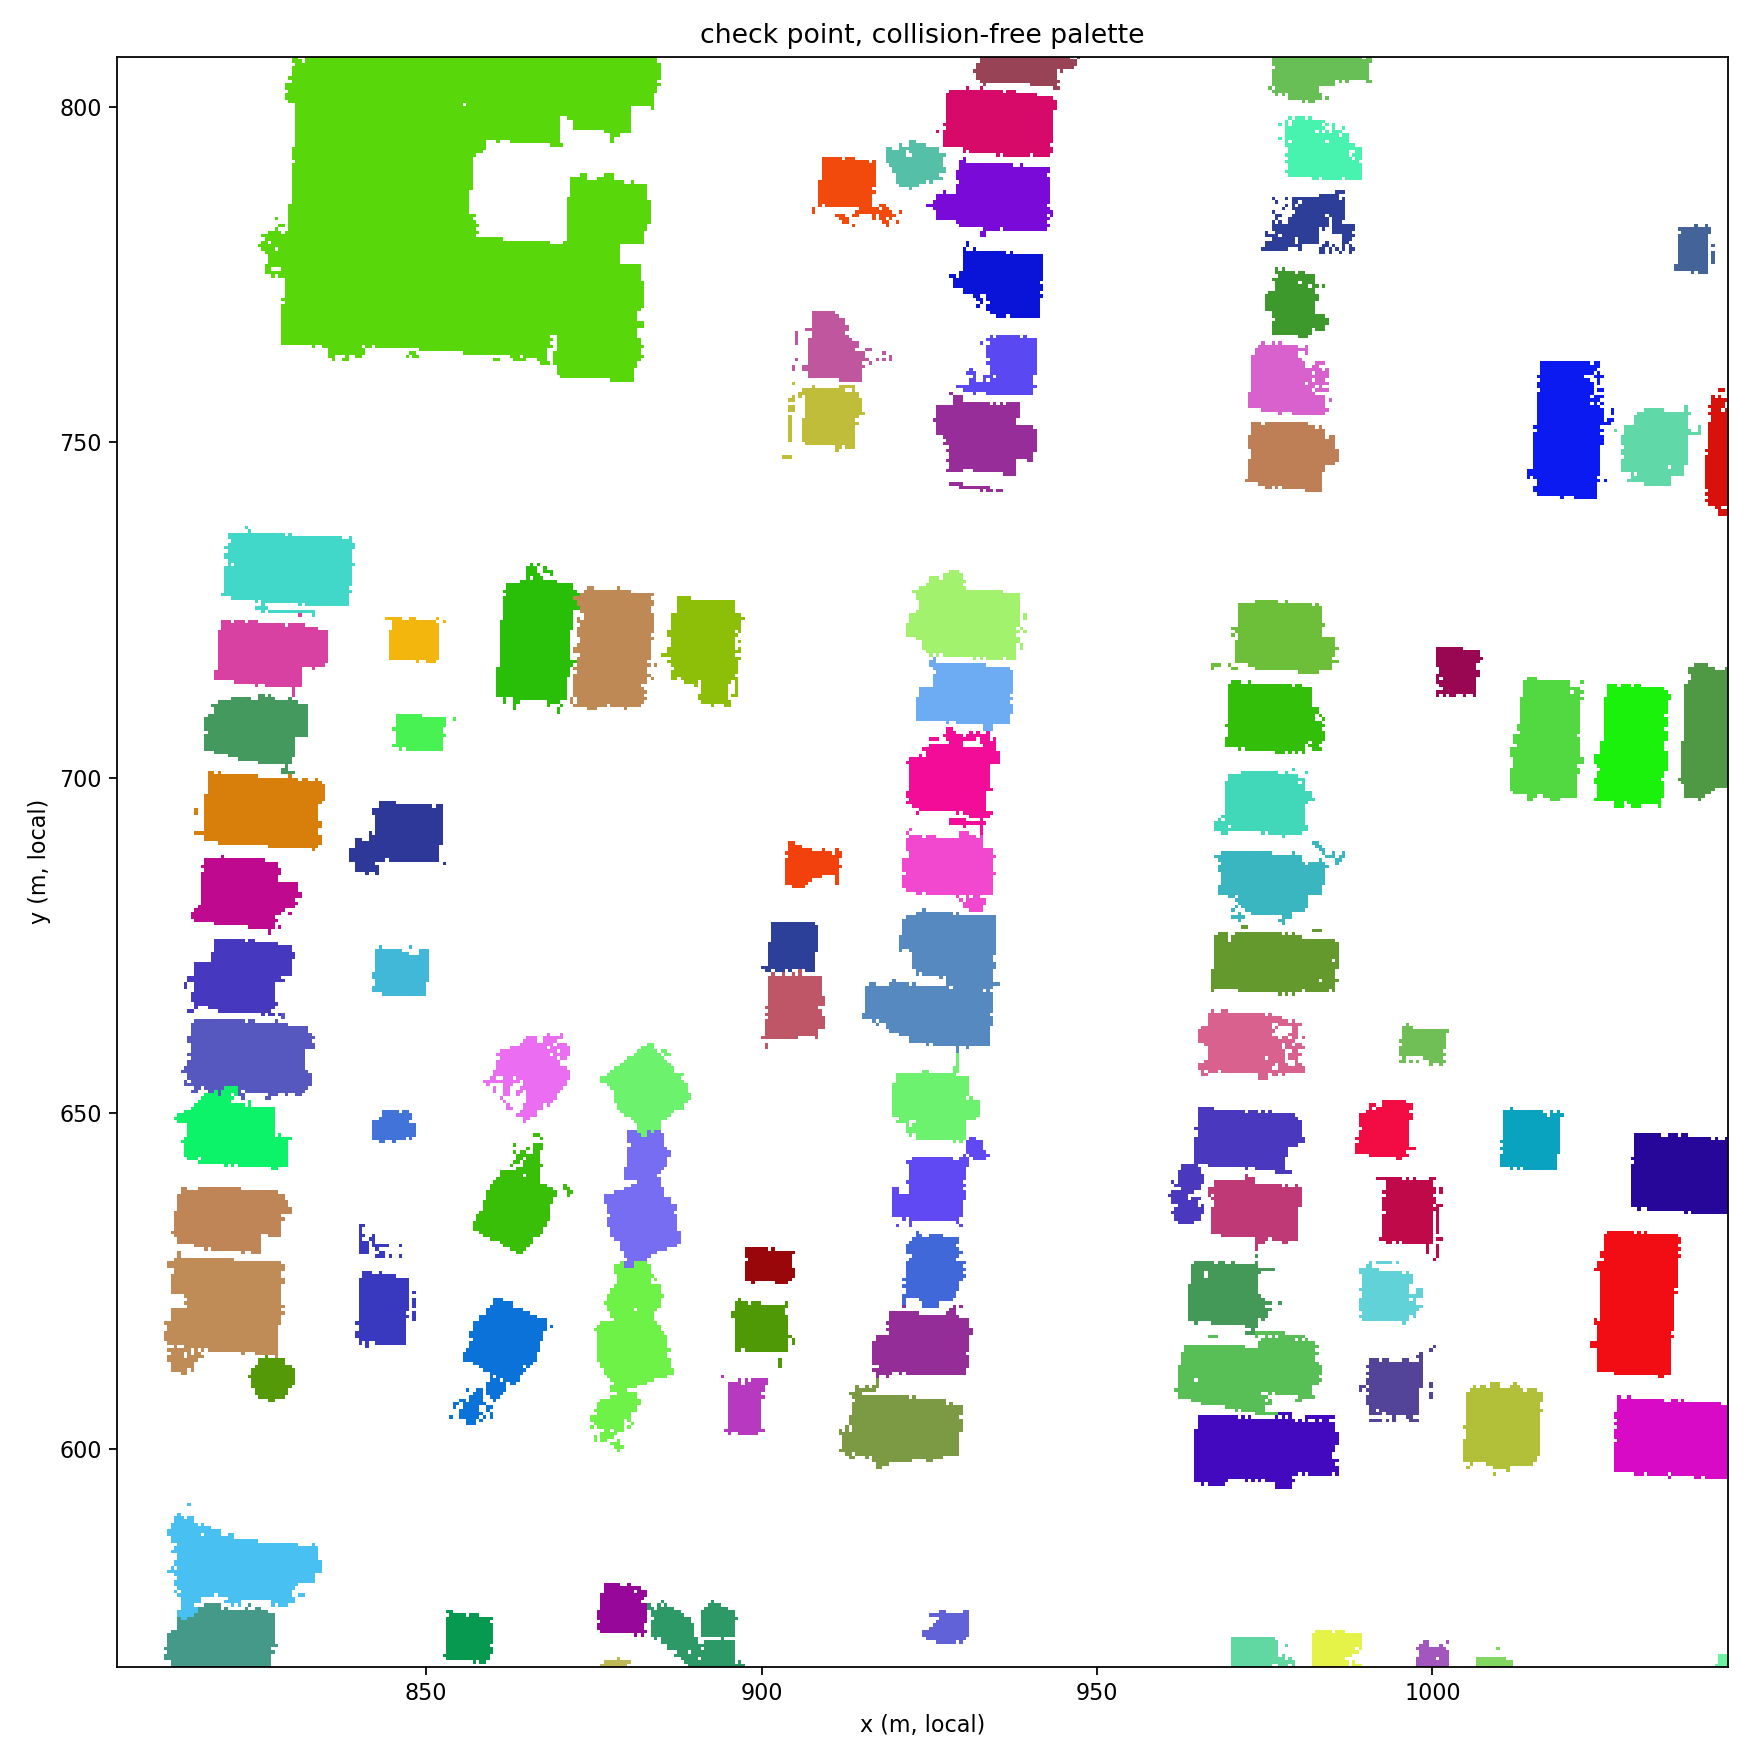
\includegraphics[width=0.72\textwidth]{figs/qa_checkpoint_rgb.png}
\caption{v2 在用户检查点的复查图（每个实例随机配色，颜色仅用于区分相邻实例，
颜色本身不代表对错）：此处正是 v1 把一排独栋串成同一实例的位置，
v2 中这排楼已各自成块、编号互不相同。}
\label{fig:checkpoint}
\end{figure}

\begin{plainbox}[：模块 3 小结]
\begin{itemize}
\item 把 863 万建筑点投进 0.5 m 方格纸，每格 $\geq2$ 点才算占据（掐死``一点桥''），
      同时每格记下最高点高程 $z_{\max}$ 备用。
\item 8-连通标记得到初步楼块；补洞改为逐块``只填包围洞''，
      \textbf{坚决不用闭运算}——v1 的欠分割事故证明：闭运算约 2 m 的桥接能力
      正落在本区 1.5--2.5 m 的侧院区间内，实测把成排独栋焊成了一个实例。
\item 遗留问题：仍有一批块粘着多栋楼。下一模块：怎么发现它们、怎么拆开。
\end{itemize}
\end{plainbox}

\newpage
\section{模块 4 · 步骤 2 下篇：把粘连的楼拆开——marker 分水岭与碎片吸收}

模块 3 结束时，我们有了一批初步楼块，其中一部分仍然``一块粘着好几栋楼''：
有的楼确实靠得太近，0.5 米格子上只隔一两格；有的被零星错点或伸过来的树枝搭了桥。
闭运算已经被我们废掉了，这些粘连不是闭运算造成的，
而是\textbf{真实数据里就存在的接触}。本模块解决两个问题：
\textbf{怎么发现}哪些块粘着多栋楼？\textbf{在哪里下刀}把它们分开？

\subsection{发现粘连：腐蚀取``核''}

工具还是模块 3 介绍过的\textbf{腐蚀}（黑色区域向内削一圈），但这次拿它当探测器用。
对每个楼块，用半径 1.5 米的圆盘做腐蚀——把块的边界向内削掉 1.5 米。直觉是：

\begin{itemize}
\item 一栋正常的楼（宽 8--15 米）削掉一圈后，中间还剩一大块——剩下的部分叫\textbf{核（core）}；
\item 两栋楼若只靠一条\textbf{窄于约 3 米}的``细脖子''相连（两侧各削 1.5 米），
      削完后脖子断开，剩下\textbf{两个分离的核}；
\item 削剩的零星小渣不算核——核的面积必须 $\geq 6$ 平方米才算数
      （否则屋顶边缘的毛刺也会被当成``第二栋楼''）。
\end{itemize}

于是判据非常干净：\textbf{一个块腐蚀后剩几个合格的核，就估计它里面有几栋楼}。
合格核不足 2 个的块（剩 1 个核，或窄楼被整个削没、0 个核）一律不拆、原样保留；
出现 $\geq 2$ 个核的块被送进下一小节拆分。顺带把单位换算清楚：
$6$ 平方米 $= 24$ 个 $0.5$ 米格子，门槛取在``明显小于最小目标建筑
（20 m\textsuperscript{2}）、又远大于边缘毛刺''的位置。

\begin{figure}[H]
\centering
\begin{tikzpicture}[scale=0.55]
% 原块：两矩形+细脖子
\begin{scope}
\fill[blue!40] (0,0) rectangle (4,3);
\fill[blue!40] (6,0.2) rectangle (10,3.2);
\fill[blue!40] (4,1.2) rectangle (6,2.0);
\node[font=\small] at (5,-0.9) {一个连通域：两栋楼被``细脖子''连着};
\end{scope}
% 腐蚀后
\begin{scope}[xshift=12.5cm]
\fill[blue!40, opacity=0.25] (0,0) rectangle (4,3);
\fill[blue!40, opacity=0.25] (6,0.2) rectangle (10,3.2);
\fill[blue!40, opacity=0.25] (4,1.2) rectangle (6,2.0);
\fill[blue!80] (0.75,0.75) rectangle (3.25,2.25);
\fill[blue!80] (6.75,0.95) rectangle (9.25,2.45);
\node[font=\small, blue!60!black] at (2,2.7) {核 1};
\node[font=\small, blue!60!black] at (8,2.9) {核 2};
\node[font=\small] at (5,-0.9) {腐蚀 1.5 m 后：脖子断了，剩两个核};
\node[font=\small] at (5,-1.7) {$\Rightarrow$ 判定``这块里有两栋楼''};
\end{scope}
\end{tikzpicture}
\caption{腐蚀取核：窄于约 3 米的连接经不起两侧各削 1.5 米；核的个数用于估计楼的栋数。}
\label{fig:erosion-core}
\end{figure}

\subsection{在哪里下刀：marker 分水岭}

知道了``这块里有两栋楼''，还得决定\textbf{分界线画在哪}。这时高度信息登场了
——模块 3 栅格化时，我们给每个格子存了``格内最高点高程 $z_{\max}$''，
现在它拼成一张\textbf{高度图}。关键观察：

\begin{center}
\fbox{\parbox{0.92\textwidth}{\centering
两栋楼即使在平面上粘着，\textbf{接缝处的高度通常塌下去}：
屋顶是块内最高的地方，而楼间的间隙里多半只有矮灌木、栅栏、地面或搭桥的零星点
——沿着``从一栋楼走到另一栋楼''的路径看高度，中间通常有一段\textbf{低谷}。
理想的分界线，就应该沿着这条高度低谷走。说``通常''而不说``必然''是有分寸的：
若伸进缝里的树枝比屋檐还高、或零星高错点把低谷抬了起来，低谷会变浅甚至消失，
边界就可能切偏——这类残余错误由人工抽查和模块 6 的``缝内地面命中''仲裁兜底。
}}
\end{center}

\textbf{分水岭算法（watershed）}正是把这个直觉自动化的经典工具（模块 2 提到的
Beucher \& Meyer 1993）。它把一张图当作\textbf{地形}来看，往里灌水：
水从各个盆地底部涨起，水位同步上升，\textbf{两片来自不同盆地的水相遇时，
在相遇处筑一道坝}——所有的坝连起来就是分割边界。

两个实现细节（也是导师可能追问的点）：

\textbf{（a）为什么用 $-z_{\max}$（高度取负）当地形？}
分水岭在``盆地''里灌水、在``山脊''上筑坝。我们想要的边界在\textbf{高度低谷}，
所以把高度整体取负、上下翻转：翻转后，高高的屋顶变成了深盆地（水源所在），
楼间低谷翻成了山脊——坝沿着山脊筑，即\textbf{边界倾向沿两楼之间高度较低的分隔带走}
（在平坦或有噪声的地方，坝的位置会有几个格子的摆动，不保证严格踩在绝对最低点的连线上）。

\textbf{（b）为什么要 marker（指定水源）？}
经典分水岭让\textbf{每一个}局部洼地都自己冒水，屋顶上随便一个烟囱、一段屋脊造成的
小起伏都会多出一片水——结果是块被切得粉碎（过分割）。
\textbf{marker 控制版}只允许指定的位置冒水：我们把上一小节的\textbf{核}当水源，
几个核就几片水，块的\textbf{主体}恰好按核数分开。两个补充细节：
其一，灌水范围被限制在原块内部（外面不归它管）；
其二，补洞补出来的格子没有点、也就没有实测高度，程序把它们赋成``极高的隔墙''参与灌水
——水最后才漫过去，通常顺势并入相邻水域；万一存在完全被隔死、水到不了的死角，
程序不强行分配，给它单独编号（实践中极少发生）。

\begin{figure}[H]
\centering
\begin{tikzpicture}[scale=0.75]
% 高度剖面
\draw[->] (0,0) -- (13.2,0) node[right,font=\small] {沿剖面位置};
\draw[->] (0,0) -- (0,3.6) node[above,font=\small] {高度 $z_{\max}$};
\draw[thick, blue!70!black]
  (0.3,0.4) -- (1.0,2.6) -- (2.6,3.0) -- (4.4,2.5) -- (5.4,0.9)
  -- (6.6,0.7) -- (7.6,1.0) -- (8.4,2.8) -- (10.4,3.1) -- (11.8,2.4) -- (12.6,0.5);
\node[font=\small, blue!70!black] at (1.2,3.35) {楼 A 屋顶};
\node[font=\small, blue!70!black] at (11.9,3.45) {楼 B 屋顶};
\node[font=\small] at (6.6,0.28) {楼间低谷（灌木/地面/桥接点）};
\draw[red!70!black, very thick, dashed] (6.6,0) -- (6.6,3.5);
\node[font=\small, red!70!black, align=center] at (6.6,3.85) {分水岭筑坝处 = 分界线};
% 水源标记
\fill[green!60!black] (2.6,3.0) circle (3pt);
\node[font=\scriptsize, green!40!black] at (2.9,2.55) {核 1（水源）};
\fill[green!60!black] (10.4,3.1) circle (3pt);
\node[font=\scriptsize, green!40!black] at (10.1,2.65) {核 2（水源）};
\end{tikzpicture}
\caption{沿``楼 A $\to$ 楼 B''的高度剖面（图中画的是\textbf{原始}高度；
算法实际在上下翻转后的地形上运行——屋顶翻成盆地、低谷翻成山脊）。
水从两个核对应的盆地涨起，相遇即筑坝：坝沿翻转后的山脊、
也就是原始高度的低谷带走。}
\label{fig:watershed}
\end{figure}

\begin{numbox}[：拆分战果]
全区共有 \textbf{168 个}连通域被检出多核并由分水岭拆开
（每次拆分的块号、拆成几份、各份面积都写进了 \texttt{splits\_log.csv} 备查）。
注意归因要分清：这 168 个是 v2 \textbf{自己}检出的多核粘连块——真实贴得近、
树枝搭桥、错点搭桥都在其中；v1 那种闭运算造成的\textbf{人为}焊接已在源头消除，
这里拆的是数据里本来就存在的粘连。168 个块共拆出 383 份、净增 215 个实例。
\end{numbox}

\subsection{防过分割的保险丝：非对称碎片吸收}

去掉闭运算、又对粘连块动刀，代价是偶尔\textbf{矫枉过正}：
屋顶被树冠遮出缺口后剩下的小角、贴着主屋的小门廊，可能孤立成小碎块。
如果放着不管，一栋楼就会变成``一大一小两个实例''（过分割）。
兜底规则是\textbf{碎片吸收}：

\begin{center}
\fbox{\parbox{0.92\textwidth}{\centering
面积 $<20$ m\textsuperscript{2} 的碎片，若在 3 米范围内存在一个面积 $\geq 50$
m\textsuperscript{2} 的``锚''实例，且两者的中位高程差 $\leq 3$ 米，则并入该锚。
}}
\end{center}

三个条件各管一件事：\textbf{面积门槛}保证只有``碎片并整楼''会发生
——两栋各 50 m\textsuperscript{2} 的真实小房子谁也吸收不了谁，
这就是``\textbf{非对称：只许小并大}''的含义，它把吸收机制自己制造欠分割的风险压到最低
（说``最低''而非``零''：一间贴着大楼、高度相近、不足 20 m\textsuperscript{2}
的真实小附属确实会被并入——本项目把这类当作主楼的附属结构，属可接受的取舍，
人工抽查也覆盖这类案例）；\textbf{3 米距离}指碎片到锚实例最近格子的平面距离
（实现上含半格容差；若周围有多个合格的锚，取\textbf{最近}的那一个，无并列歧义）；
\textbf{高程相容}比较两者的\textbf{中位高程}（把各自所有点的高程从小到大排队取正中间那个值
——不被烟囱等零星极端点带偏），拦住``隔着高差硬并''的错误，
例如把 10 米高的树冠碎片并进 4 米高的平房。

\subsection{收尾三件事：丢渣、捡孤儿、发号}

\textbf{（1）丢渣}：吸收后仍孤立、面积 $<20$ m\textsuperscript{2} 的小块按噪声丢弃
——这是项目的\textbf{最小制图面积}取舍：比单车库还小的独立结构
（工具棚、狗屋、凉棚）不在本项目的建模目标内，而零星错点凑成的假团块又恰好多在
这个尺寸段，一刀切最干净。
\textbf{（2）捡孤儿}：模块 3 的占据规则（每格 $\geq2$ 点）丢掉了稀疏格子里的点，
其中有些其实是真屋顶的边缘。现在把这些``孤儿点''挂回平面距离 \textbf{1.5 米}（$=3$ 个格子）内\textbf{最近}的实例格
（距离按格网量取，最近者唯一，不存在并列歧义）；1.5 米内没有实例的，
维持无主（instance\_id = 0），不强行认领。窄缝里两楼几乎等距时，
个别边界点可能挂错家门——这是逐点级的小误差，不改变实例结构，由抽查覆盖。
\textbf{（3）发号}：所有实例按面积从大到小重新编号 1, 2, 3, \dots，
每个点的编号作为新增属性 \texttt{instance\_id} 写回点云文件。

\subsection{结果与人工验收}

\begin{numbox}[：步骤 2 最终产出]
\textbf{2{,}296 个建筑实例}（候选），编号 1--2296，逐点写入
\texttt{buildings\_instances.laz}；随机抽查窗口与 v1 出错点的复查图作为质检产物存档。
对账线索：初步连通域数 $+$ 拆分净增 215 $-$ 吸收合并数 $-$ 丢渣数 $= 2{,}296$；
拆分明细逐块存档（\texttt{splits\_log.csv}），吸收与丢渣的逐项计数在运行日志中，重跑可复现。
\end{numbox}

\begin{warnbox}[：显示上的一个小教训——``防撞色'']
最初把实例编号直接用连续色带显示（编号 1 深蓝、2296 深红、中间渐变），
用户检查时发现\textbf{相邻楼的编号往往相近、颜色几乎一样}，看起来就像``同一个实例''
——白白制造了一场虚惊。之后所有实例一律改用\textbf{随机防撞色}
（每个实例随机挑一个颜色、并保证与邻居不同），并把颜色直接写进点云文件的 RGB 属性列（每个点存红、绿、蓝三个颜色数值），
在支持按 RGB 着色的查看软件里打开即见防撞色，不再依赖软件自选的色带。
这个习惯延续到了管线后面所有输出。
\end{warnbox}

\begin{figure}[H]
\centering
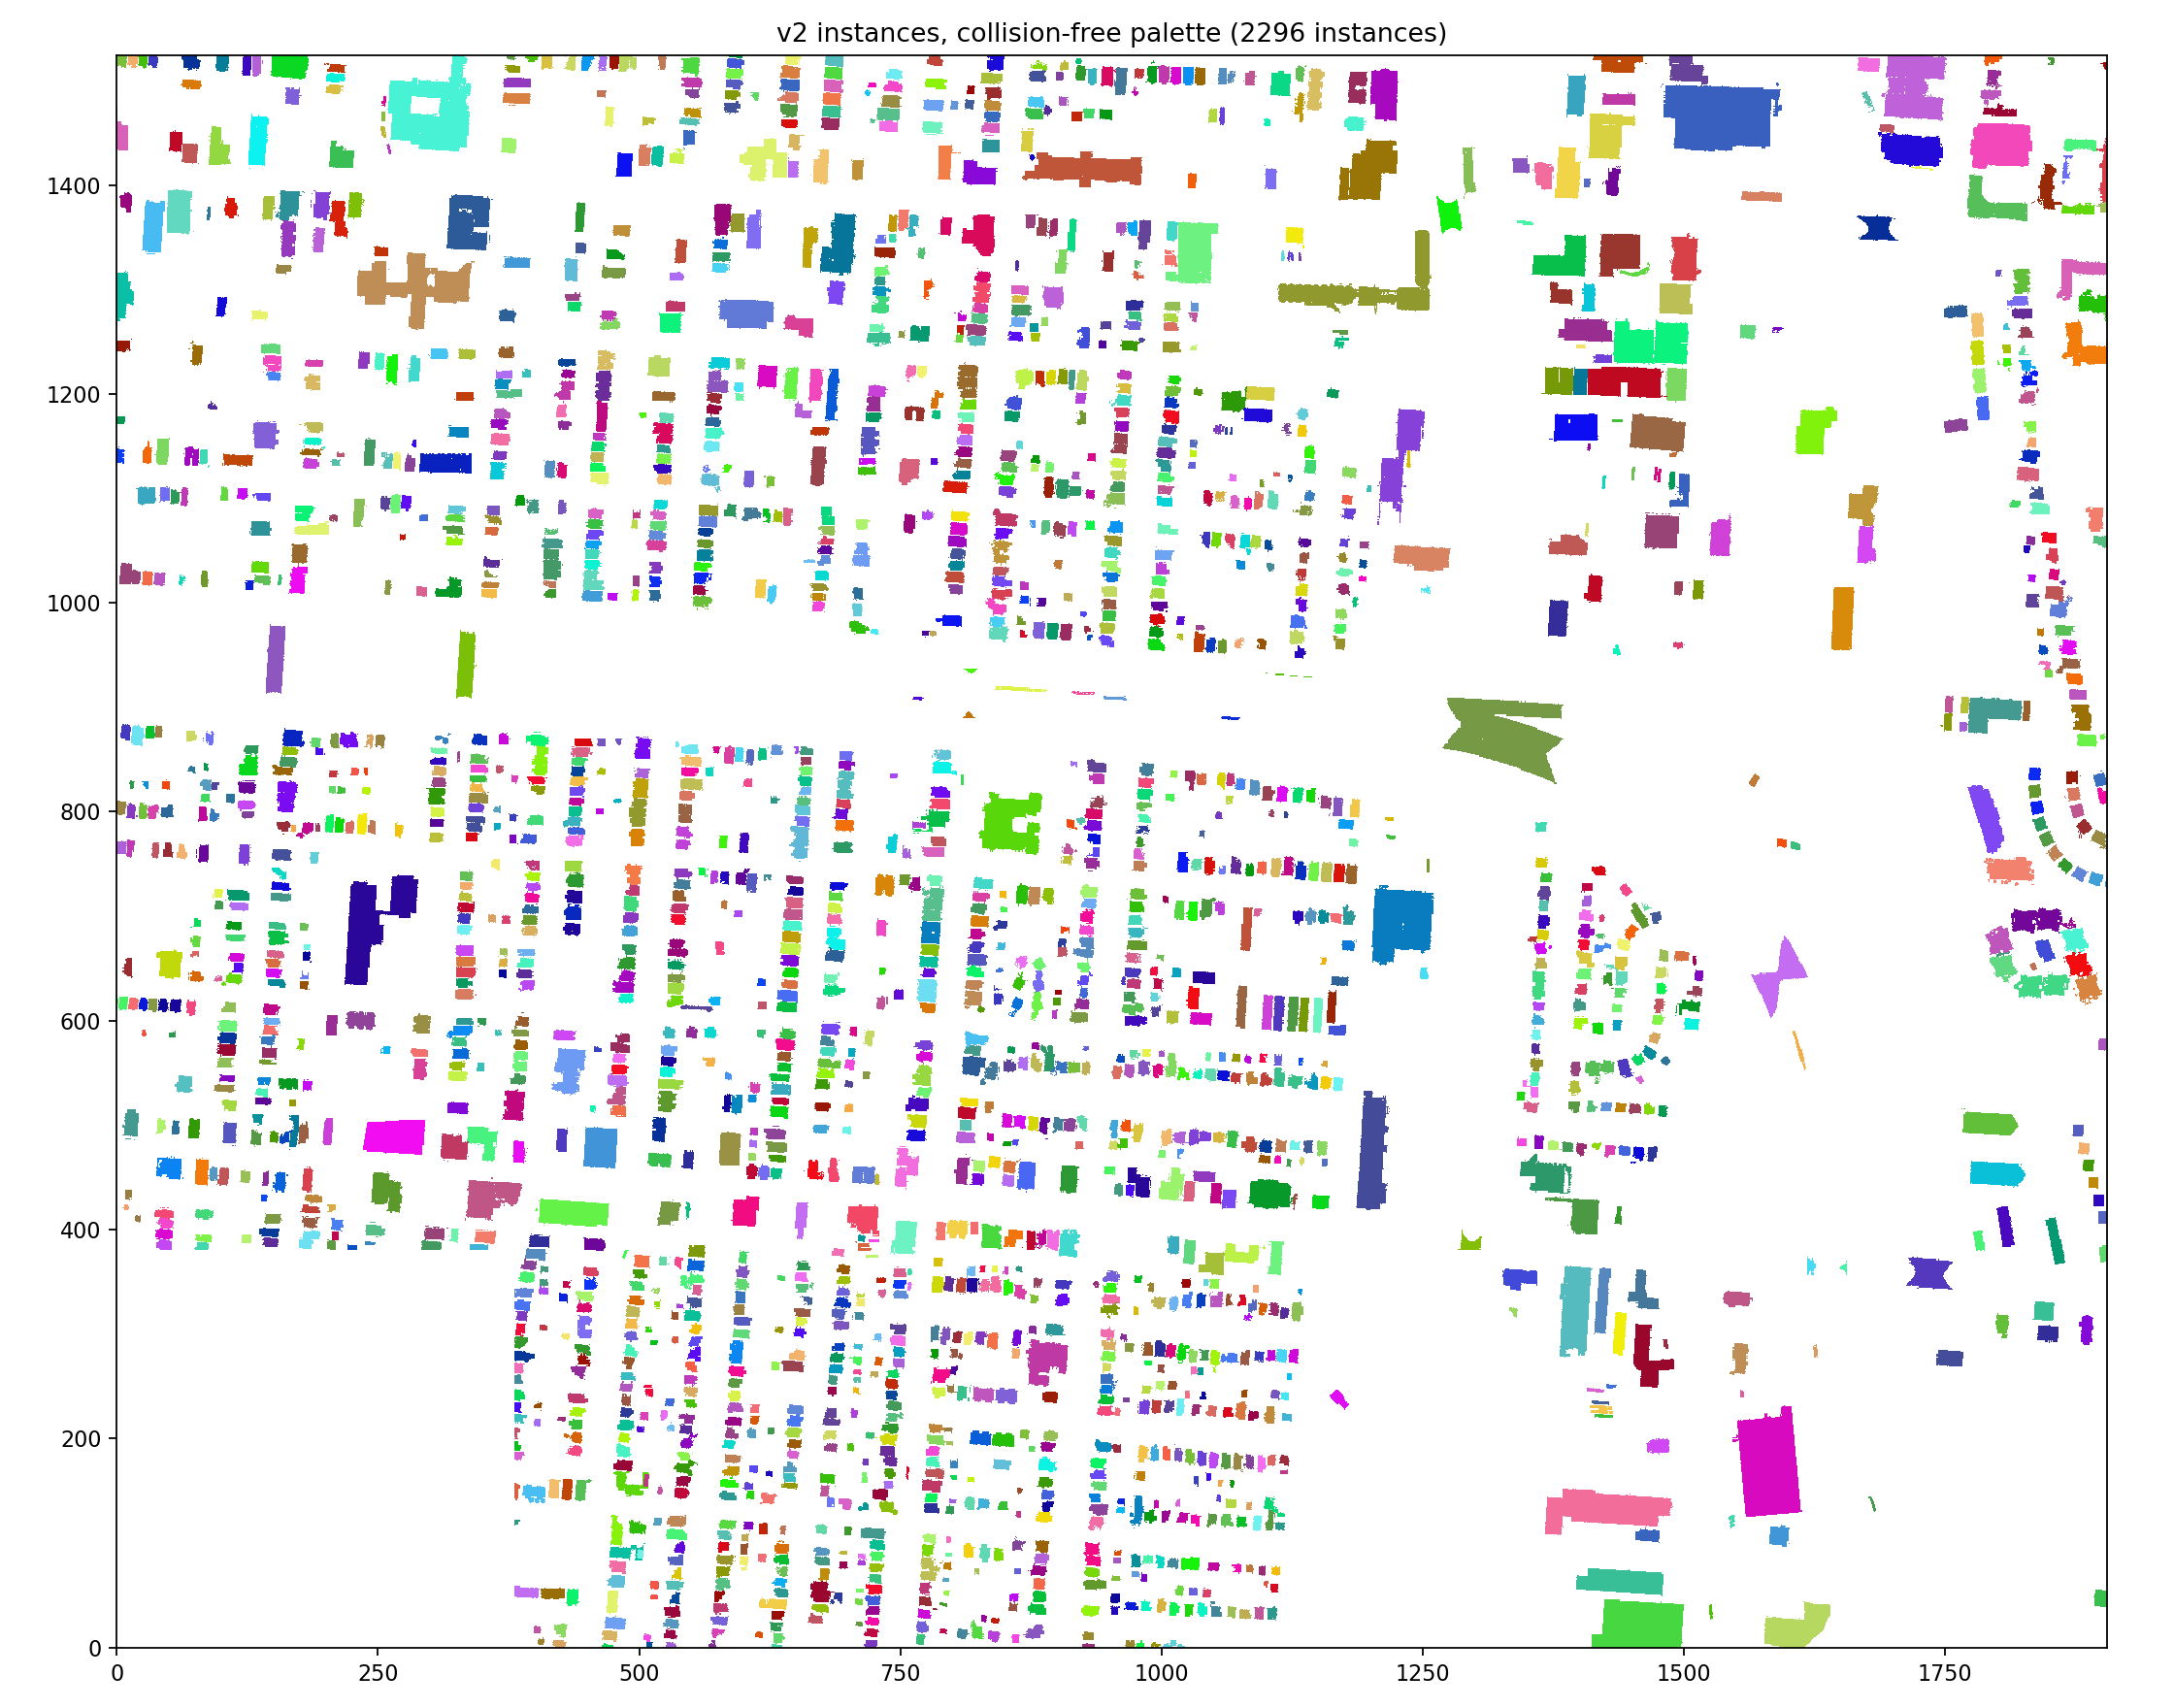
\includegraphics[width=0.9\textwidth]{figs/qa_overview_rgb.png}
\caption{步骤 2 全区总览（每实例一个防撞色）：2{,}296 个候选建筑实例。
可以看到住宅街区被整齐地逐栋分开；图中零星的大块异形目标（桥、匝道等）
正是下一模块 Gate A 要处理的对象。}
\label{fig:overview}
\end{figure}

\begin{plainbox}[：模块 4 小结]
\begin{itemize}
\item 腐蚀取核发现粘连（削 1.5 m、核 $\geq6$ m\textsuperscript{2}），
      168 个多核连通域被 marker 分水岭沿\textbf{高度低谷}拆开（383 份、净增 215）
      ——水源=核，地形=$-z_{\max}$，边界沿两楼之间高度较低的分隔带走。
\item 非对称碎片吸收（$<20$ m\textsuperscript{2} 并入 3 m 内 $\geq50$ m\textsuperscript{2}
      且高程相容的锚）兜住过分割，``只许小并大''保证它不反向制造欠分割。
\item 丢渣、捡孤儿、按面积发号后：\textbf{2{,}296 个候选建筑实例}。
      其中混着的桥、匝道、树冠、电线，交给模块 5 的 Gate A。
\end{itemize}
\end{plainbox}

\newpage
\section{模块 5 · 步骤 3：Gate A 噪声闸门——把``不是楼的东西''请出去}

步骤 2 交出了 2{,}296 个候选实例，但其中混着 RandLA-Net 错标出来的``假建筑''：
高架桥面、立交匝道、成排树冠、电力线。本模块讲这道质量闸的设计：
\textbf{先算每个实例``离地多高''和``长什么形状''，用规则捞出可疑分子，
最后由人工逐个判读定生死——每个被剔除的实例都留有原因码和证据}。

\subsection{为什么非要这道闸：假建筑不会自我暴露}

一个自然的想法是``不用管，后面重建失败的自然就是假建筑''。这个想法对桥这类目标\textbf{恰恰是错的}：
桥面、匝道本身就是平整的板，后续用数学平面去近似它们时，
比近似真屋顶还要顺利——\textbf{残差}（每个点到拟合平面的偏差）极小、平面性完美，
\textbf{全程不会触发任何报错}。换句话说，重建环节对``桥 vs.\ 楼''是\textbf{无感}的
（City3D 论文（Huang et al.\ 2022）所描述的重建机理决定了这一点：
算法只看几何，凡是平面都一视同仁）。顺带一提：蓬松的树冠倒\textbf{会}在平面拟合上露馅
——但那要等第 4 步跑完才看得到，正是模块 6 追溯修正利用的证据；
桥这种``完美平面''则永远不会自我暴露，必须现在拦。
所以清除必须发生在\textbf{进入重建之前}，而且要用\textbf{实例级}的特征
——单看一个点谁也分不清桥和楼，但看\textbf{一整个实例}的高度和形状，两者立刻露馅。
这也是荷兰 3D BAG 等生产管线的共同设计（模块 2 已介绍）。

\subsection{第一块积木：地面在哪——建一张 DTM}

要判断``实例离地多高''，先得知道\textbf{地面本身多高}。这就是
\textbf{DTM（Digital Terrain Model，数字地形模型）}：一张``每个平面位置上、
地面的高程是多少''的图。我们用第 1 步分好的\textbf{类别 2（地面）点}来建，
铺一张 1 米的方格纸，三步走：

\begin{enumerate}
\item \textbf{每格取最低值}：格内所有地面点的最低高程作为该格地面高
      （只要格内还有真实地面点，取最低值就不受少量偏高错点影响；
      万一整格都是错点，交给下一步的中值滤波兜底）；
\item \textbf{中值滤波去毛刺}：拿每格与它周围 $3\times3$ 邻域的``中间值''比较，
      偏差超过 2 米的格子（孤立的坑或尖，多半是错点造成）用中间值替换。
      ``中值/中位数''就是把一串数从小到大排队后取正中间那个——它对个别离谱值完全不敏感；
\item \textbf{补洞}：楼底下没有地面回波，这些格子是空的，用\textbf{最近的有值格}填上
      ——相当于把楼周围的地形``借''到楼底下。
\end{enumerate}

\subsection{第二块积木：离地高度 HAG}

有了 DTM，每个实例的\textbf{离地高度（HAG, height above ground）}定义为：

\begin{center}
\fbox{\parbox{0.92\textwidth}{\centering
$\mathrm{HAG} \;=\; $ 实例点云的\textbf{中位高程} $z_{50}$
$\;-\;$ 实例\textbf{周围 4 米环带内} DTM 的\textbf{第 5 百分位} $P_5$
}}
\end{center}

三个选择都有讲究（也是导师可能问的细节）：

\textbf{为什么取楼``周围''的地面，不取楼``底下''的？}
楼底下的 DTM 全是第 3 步``借''来的填补值；而环带取值时\textbf{只用原本就有
实测地面点的格子}（实测格不足 20 个时才退回填补值），可靠得多。
这个``4 米环带''的约定沿用 3D BAG 生产线（Peters et al.\ 2022）；
3D BAG 用官方轮廓定义``楼的周围''，我们没有轮廓，用实例自身外扩 4 米代替。

\textbf{什么是``第 5 百分位 $P_5$''？}把环带里所有 DTM 值从低到高排队，
取排在 5\% 位置的那个数——比``最低值''稳健（不被单个坏点带偏），
又比``平均值''偏向低处（环带里常混着台阶、缓坡、花坛，取偏低值代表``真正的地面''）。

\textbf{为什么用中位数 $z_{50}$ 代表楼高、而不用最高点？}
中位数代表``屋顶主体''的高度，不被烟囱、天线之类的零星高点绑架。

\begin{figure}[H]
\centering
\begin{tikzpicture}[scale=0.72]
% 地形线
\draw[thick, brown!70!black] (0,0.6) -- (2.2,0.5) -- (4.2,0.42) -- (9.8,0.35) -- (12.6,0.42);
\node[font=\scriptsize, brown!60!black] at (1.2,0.15) {DTM（地面高程）};
% 房子
\fill[blue!25] (5,0.4) rectangle (9,2.2);
\draw[thick] (5,2.2) -- (7,3.2) -- (9,2.2);
\fill[blue!45] (5,2.2) -- (7,3.2) -- (9,2.2) -- cycle;
% 环带
\draw[<->, green!50!black, thick] (4.95,0.9) -- (3.0,0.9) node[midway, above, font=\scriptsize] {4 m 环};
\draw[<->, green!50!black, thick] (9.05,0.9) -- (11.0,0.9) node[midway, above, font=\scriptsize] {4 m 环};
\draw[green!50!black, dashed] (3.0,0.0) -- (3.0,1.35);
\draw[green!50!black, dashed] (11.0,0.0) -- (11.0,1.35);
\node[font=\scriptsize, green!40!black] at (7,-0.25) {环带内 DTM 的 $P_5$ = ``真正的地面''};
% z50
\draw[red!70!black, dashed] (4.0,2.62) -- (10.0,2.62);
\node[font=\scriptsize, red!70!black] at (11.5,2.62) {屋顶 $z_{50}$};
% HAG
\draw[<->, thick] (4.35,0.47) -- (4.35,2.62) node[midway, left, font=\small] {HAG};
\end{tikzpicture}
\caption{离地高度：屋顶中位高程减去楼周 4 米环带内地面的 $P_5$。
规则线：$\mathrm{HAG} < 2$ 米的实例基本不可能是本项目的目标建筑
（独栋住宅一层的屋顶通常离地 3 米以上）；本区该规则实际触发 0 例。}
\label{fig:hag}
\end{figure}

规则设定为 \textbf{HAG $< 2$ 米 $\Rightarrow$ 剔除}。要说明：这是 Gate A 里
\textbf{唯一}允许自动执行的剔除——离地不足 2 米，物理上容不下本项目的目标建筑
（独栋住宅），所以它是后文``人工定罪''原则的一个明确例外。一个诚实的实测结果：
它在本区\textbf{一个实例都没触发}——步骤 2 的占据规则（每格 $\geq2$ 点）和
20 m\textsuperscript{2} 面积门槛已经把贴地的零星错标拦在了实例名单之外。
因此\textbf{实际发生的每一次剔除都过了人工的眼睛}。这条规则仍留在闸门上：
换一片语义分割表现更差的区域，它就是第一道防线。

\subsection{真正干活的两条``捞候选''通道}

本区真正的假建筑（桥、匝道、树列、电线）都\textbf{又高又像样}——HAG 拦不住它们。
它们的破绽在\textbf{形状}：

\textbf{通道一：细长体检测。}桥、走廊、电力线、树列的共同点是\textbf{细长}。
我们用``长宽比''AR 描述一个实例的形状：把实例的平面形状概括成
``最长方向的伸展 / 最宽方向的伸展''（技术上由主成分分析 PCA 计算：
找出点分布伸展最大与最小的两个方向、取两者比值——可以理解成
``给这堆点量身高和腰围，再作比''）。规则：\textbf{AR $\geq 5$ 的实例进入候选名单}。
全区捞出 \textbf{18 个候选}——注意，\textbf{候选不等于剔除}：
真实世界里联排长条建筑同样细长，机器分不清``细长的桥''和``细长的楼''，
所以最终裁决交给人：逐个渲染出俯视图和高度剖面、目视判读。
结果：\textbf{8 个剔除}（4 个桥面/走廊构筑物、1 个线性匝道、1 列行道树、2 条电力线），
\textbf{10 个保留}（确为真实的长条建筑）。

\textbf{通道二（Gate A2）：折带检测。}用户在抽查中发现了通道一的漏网之鱼：
\textbf{折叠形态的匝道}——Z 字形、领结形的立交匝道，局部是细带，
但整体折叠得很紧凑，``身高腰围比''AR 反而不大，从通道一的指标缝里溜了过去。
对策是换用两个\textbf{对折叠免疫}的判定量：\textbf{solidity}（充实度）与
\textbf{elong}（伸长指标，由``最宽处宽度''导出）——

\begin{itemize}
\item \textbf{充实度 solidity} = 实例面积 $\div$ 凸包面积。\textbf{凸包}可以想象成
      ``用一根橡皮筋把整个形状箍起来''得到的最小凸多边形。
      折带只占它凸包的一小部分（solidity 常在 0.4--0.6），
      而正经建筑基本填满自己的凸包（$>0.75$）；
\item \textbf{最宽处宽度}（由距离变换 EDT 计算：找出形状内部\textbf{离边界最远}的点，
      它到边界距离的 2 倍就是形状``最宽的地方''）。折带无论怎么折，
      最宽处也只有一条路的宽度；真建筑的最宽处就是楼身宽。
      配套的伸长指标 elong = 面积 $\div$ 最宽处宽度$^2$：同样面积下越``带状''值越大。
\end{itemize}

为什么 AR 抓不住折带、这两个量抓得住？折叠让整体外形变紧凑，``身高腰围比''AR
随之变小；但无论怎么折，折带都\textbf{填不满自己的凸包}（solidity 低）、
\textbf{局部也宽不起来}（同样的面积摊在窄带上，elong = 面积 $\div$ 最宽处$^2$ 变大）
——两个量从不同侧面锁定``带状''本性，互为补网：实测两块方正的桥板
solidity 高达 0.88--0.91，正是靠 elong $\geq3.5$ 落网的。

规则：面积 $\geq 400$ m\textsuperscript{2} 且（solidity $\leq 0.72$ 或 elong $\geq 3.5$）
进入候选，再次逐个目视判读。三个阈值不是文献值，而是在全区形状特征表的分布上定的
（\texttt{shape\_features.csv} 逐行记录了 1{,}711 个 $\geq80$ m\textsuperscript{2}
实例的 solidity/最宽处/elong）：全区 \textbf{96.4\%} 的实例 solidity $>0.75$，
0.72 取在建筑主体与已知折带样本（0.62、0.66）之间的空档；
400 m\textsuperscript{2} 的面积门槛避免把普通的小型 L 形/U 形住宅大量捞进候选
（目标折带全都远大于此）。按此规则命中 \textbf{25 个}候选，外加 2 个点名复查的编号；
逐个判读后\textbf{剔除 5 个}（1 个铁路走廊上的 Z 字折带构筑物、2 个领结形匝道、
2 块桥板），其余确认为真实的大体量建筑、保留。

\begin{figure}[H]
\centering
\begin{tikzpicture}[scale=0.5]
% 折带
\begin{scope}
\draw[line width=7pt, blue!50, line cap=round]
  (0,0) -- (3.4,0.5) -- (0.9,2.0) -- (4.2,2.6) -- (1.5,4.0);
\draw[red!70!black, thick, dashed] (-0.4,-0.6) -- (4.8,0.2) -- (4.8,3.1) -- (1.1,4.6) -- (-0.4,2.1) -- cycle;
\node[font=\small, align=center] at (2.2,-1.6) {折带匝道：面积只占\\ 凸包（红虚线）一小部分\\ solidity 低、最宽处窄};
\end{scope}
% 建筑
\begin{scope}[xshift=10cm]
\fill[blue!50] (0,0) rectangle (4,3) (4,0.8) rectangle (5.2,2.4);
\draw[red!70!black, thick, dashed] (-0.15,-0.15) rectangle (5.35,3.15);
\node[font=\small, align=center] at (2.6,-1.6) {真建筑：基本填满凸包\\ solidity 高、最宽处 = 楼身宽};
\end{scope}
\end{tikzpicture}
\caption{Gate A2 的两个抗折叠判定量（solidity 与 elong）：折带无论怎么折，
``填不满凸包、局部宽不起来''的本性不变；方正的桥板则靠 elong 落网。}
\label{fig:solidity}
\end{figure}

\subsection{设计原则与审计产物：规则捞人，人来定罪}

Gate A 全程贯彻一条原则：\textbf{自动规则只负责``把可疑分子捞出来''，
剔除的最终决定权全部在人工判读}。理由很朴素：任何形状规则都存在
``长得像桥的楼''（细长联排）与``长得像楼的桥''；而两条通道合计候选不足 50 个
（通道一 18 个，通道二 25+2 个，两者不重叠——通道二不再复查通道一已定案的实例），
逐个看图也就半小时的事——用最便宜的人力换零误杀。
（唯一的自动例外 HAG$<2$ 米，其物理依据前文已述，且本区触发 0 例。）

配套的\textbf{可审计}产物（导师问``你怎么保证没删错''时的底气）：

\begin{itemize}
\item \texttt{instances\_gateA.csv}：全部实例逐行记录（点数、面积、地面高、
      离地高度、长宽比、宽度、判定），每个剔除都带\textbf{原因码}
      （如 \texttt{reject\_reviewed\_bridge\_corridor}）；
      配套的 \texttt{shape\_features.csv} 存有全部 $\geq80$ m\textsuperscript{2}
      实例的 solidity/最宽处/elong——Gate A2 每个候选为何入选，均可据表复核；
\item \texttt{noise\_removed.laz}：被剔除实例的点\textbf{不是删除而是移仓}
      ——单独存档，随时可以在 CloudCompare 里回看核对；
\item 三张判读证据图（细长候选逐个渲染、形状候选逐个渲染、高度剖面三连查），
      判读结论直接写在代码里（哪个编号、什么原因），完全可复查。
\end{itemize}

\begin{numbox}[：Gate A 战果]
剔除 \textbf{13 个}非建筑实例：4 个桥面/走廊构筑物、1 个线性匝道、
2 个领结形折带匝道、1 个 Z 字折带（铁路走廊上的构筑物，原因码沿用
\texttt{ramp\_zigzag}）、2 块桥板、1 列行道树、2 条电力线。
（原因码计数：\texttt{bridge\_corridor}$\times$4、\texttt{ramp\_linear}$\times$1、
\texttt{ramp\_bowtie}$\times$2、\texttt{ramp\_zigzag}$\times$1、
\texttt{bridge\_deck}$\times$2、\texttt{tree\_row}$\times$1、
\texttt{powerline}$\times$2，合计 13。）
实例数 $2{,}296 - 13 = \textbf{2{,}283}$。
\end{numbox}

\begin{figure}[H]
\centering
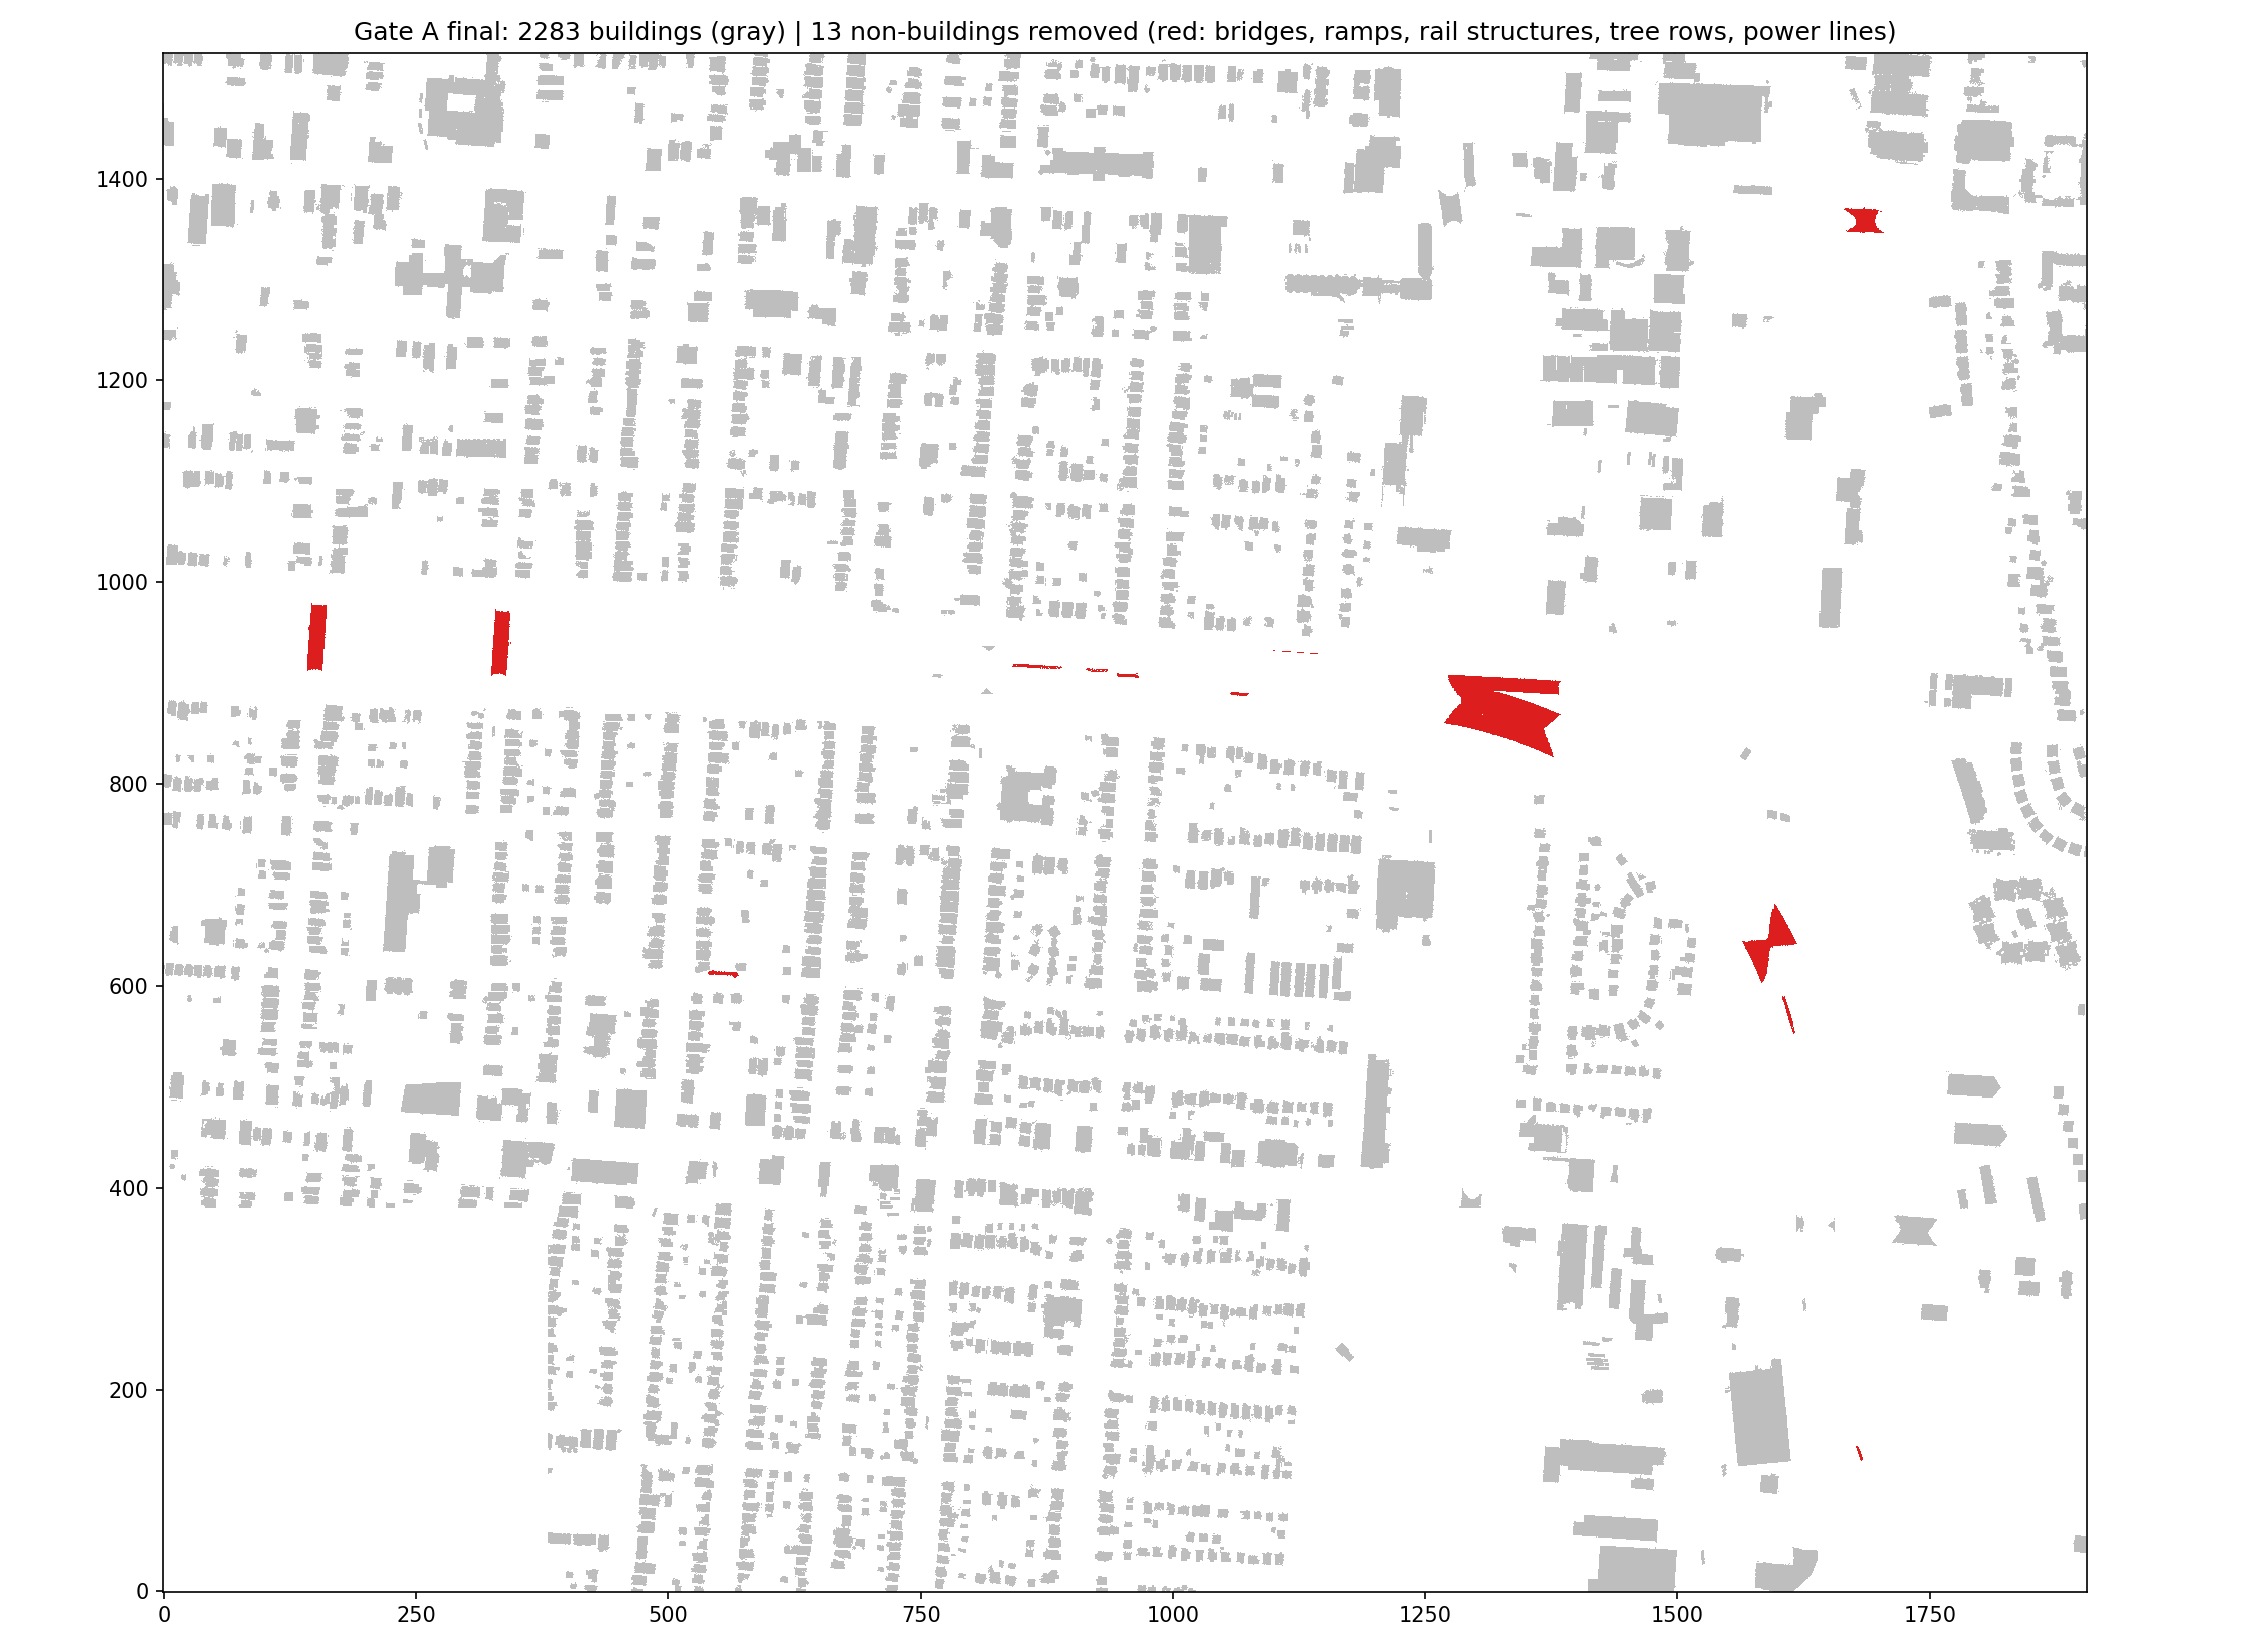
\includegraphics[width=0.95\textwidth]{figs/qa_gateA.png}
\caption{Gate A 审计总图：灰色 = 保留建筑；红色 = 剔除的非建筑。
红色斑块呈带状排列——经与道路/铁路位置核对，剔除对象集中在高速公路与铁路走廊沿线
（图中未叠加路网；做 PPT 时可补一层路网底图佐证）。}
\label{fig:gateA}
\end{figure}

\begin{plainbox}[：模块 5 小结]
\begin{itemize}
\item 假建筑在重建阶段不会自我暴露（桥比楼还平），必须在重建前用实例级特征清除。
\item 三层特征：离地高度 HAG（DTM + 4 m 环 $P_5$，3D BAG 约定）、
      细长度 AR、抗折叠判定量（solidity + elong）。
\item 规则只捞候选、人工定罪、原因码 + 移仓存档全程可审计：
      $2{,}296 \to 2{,}283$。但故事没完——还有两类更隐蔽的错误
      要靠\textbf{后续步骤反馈回来}才能发现，这就是模块 6。
\end{itemize}
\end{plainbox}

\newpage
\section{模块 6 · 追溯修正与最终台账：闸门允许被更强的证据推翻}

模块 5 结束时实例数是 2{,}283，但你在前面已经多次看到最终数字是 \textbf{2{,}267}。
差额来自两批\textbf{追溯修正}（retroactive correction）：
Gate A 判决之后，管线继续往下跑，\textbf{下游步骤算出了 Gate A 当时没有的更强证据}，
据此回头推翻了一批早先的判决。本模块讲这两批修正、一次被否决的``聪明主意''，
以及最后的逐项对账——这部分是汇报里最能体现方法论成熟度的内容。

\subsection{为什么闸门要允许``往回开''}

Gate A 手里只有实例的\textbf{高度}和\textbf{平面形状}。有两类冒牌货靠这两样看不出来：

\begin{itemize}
\item \textbf{茂密的树冠团}：又高（$>$5 米）又紧凑（俯视近圆形），高度、形状都像一栋小楼；
\item \textbf{被树``桥接''的连体楼}：两栋楼中间隔着大树，树冠被错标成建筑点、
      恰好把两栋楼连成一片——看起来就是一栋大楼（步骤 2 的漏网欠分割）。
\end{itemize}

它们的破绽要等\textbf{下游}才显形：第 4 步平面提取会发现树冠``拟合不出像样的平面''；
后续轮廓处理会发现连体楼的屋顶``裂成两大块''。设计选择是：
\textbf{不假装闸门一次判对，而是把下游的新证据回传，逐案重审、修正、记录}
——审计表里这类判决的原因码都带 \texttt{retro}（追溯）字样，全程可查。

\subsection{追溯修正一：22 个树冠假实例}

\textbf{新证据有两条}，都是可计算的分数：
（a）\textbf{植被上下文}：对每个提取出的平面，统计``它所占的 1 米格子（向外扩 1 格）内、
高程落在该平面上下 2 米窗口里的类别 5（植被）点数''与平面自身点数之比。
真屋面身边的植被在窗口之外（比值 $\approx0$）；树冠拟出来的假面则整个泡在同一团
类别 5 点云里（比值远大于 1，记为``植被嫌疑面''）。
（b）\textbf{平面性反馈}：树冠蓬松，点大量归不进任何平面。
把每个实例的``无平面可归的点 $+$ 植被嫌疑面上的点''加起来除以实例总点数，
占比 $\geq 0.90$（几乎整个实例都不像正经屋顶）即成为\textbf{实例级候选}。

按此规则全区捞出 \textbf{24 个候选}，\textbf{逐个人工目验}（俯视图 + 高度剖面）：
\textbf{22 个确认为树冠、整实例剔除}；\textbf{2 个救回}——树下工具棚、单坡车棚这类
真实结构，点稀疏又埋在植被堆里，分数高到 0.94--0.95，目验却一眼可辨是人造物。
连同平面级复核中救下的另 4 个，共 \textbf{6 个实例进入白名单}永久保护。
这 6 个救回案例正说明``规则捞人、人来定罪''不是走过场。
被剔除的 22 个实例照例\textbf{移仓存档}（\texttt{veg\_reclassified.laz}），
原因码 \texttt{reject\_vegetation\_retro} 写回审计表；两项证据分数逐实例/逐面存于
\texttt{instance\_veg.csv} 与 \texttt{plane\_veg.csv}，每个判读都可据表复核。

\subsection{插曲：一个被数据否决的``聪明主意''（负结果）}

处理树冠问题时出现过一个诱人的想法，最终被我们\textbf{用实测数据否决}。
汇报时值得专门讲——它展示``选型靠证据、不靠直觉''。

先补一个知识点：一束激光可以有\textbf{多次回波}（multiple returns）。
激光打到树叶时一部分能量反射（第 1 次回波）、其余能量穿过缝隙继续前进，
可能再打到枝叶（第 2 次）、最后打到地面（最后一次）。所以每个点都带着
``这是第几次回波 / 共几次''的属性。本讲义说的\textbf{中间回波}，操作定义是
``\textbf{回波序号 $<$ 总回波数}''——即多次回波脉冲里\textbf{非最后一次}的回波
（多回波的第 1 次也算在内；不算的只有单次回波与每束脉冲的最后一次）。
树冠的典型特征就是大量中间回波：实测本区\textbf{全部植被（类别 5）点}中
\textbf{94.8\%} 是中间回波，而\textbf{全部被标为建筑（类别 6）的点}中只有
\textbf{10.4\%}——注意这两个比例的分母不同，后面还会用到这一点。

诱人的想法随之而来：\textbf{在单体化之前，把中间回波点统统删掉}，
树冠不就从源头消失了？实测评估给出了两条相反的证据：

\begin{enumerate}
\item \textbf{代价大得离谱}：拿一栋干净的人字顶住宅做案例试验，删中间回波会损失
      该楼 \textbf{9.3\%} 的点（428/4{,}579，图~\ref{fig:echo} 左、中），
      而且\textbf{全部集中在屋檐一圈}——激光束扫到屋檐边缘时会``劈成两半''
      （一半打屋檐、一半继续打到地面），屋檐点因此常是``第 1 次/共 2 次''回波，
      按上面的操作定义正属于中间回波。而屋檐一圈正是建筑\textbf{外轮廓的核心证据}，
      删它等于自毁轮廓。
\item \textbf{收益小得可怜}：对一个真实的树冠污染团（曾被错标成建筑的实例）实测，
      删中间回波只能去掉其中 \textbf{16\%} 的树点（图~\ref{fig:echo} 右）
      ——84\% 的污染原样留下。为什么与 94.8\% 差这么远？这是一次典型的
      \textbf{选择偏差}（selection bias）：我们面对的不是``全体树点''，
      而是\textbf{先被 RandLA-Net 错标成建筑}的那部分树点；模型恰恰倾向把
      ``回波上像表面''的树点——单次或末次回波——错标成建筑，
      于是这个被筛出来的子集\textbf{天然缺乏}中间回波特征。
      94.8\% 描述的是没被错标的大多数，拿它推断被错标的少数，就掉进了坑里。
\end{enumerate}

结论：点级回波预过滤\textbf{否决}——两个案例试验的分母各不相同（一栋楼的全部点 vs
一团污染的树点），不能直接相减比较，但方向一致且都致命：真目标出现集中于屋檐的
\textbf{结构性}损伤，假目标的大头却删不掉。回波属性改记为\textbf{面级}判别的
候选辅助特征（``面级''＝先对一个屋顶平面汇总其内部点的中间回波占比、再整面判断
——目前记录在案、\textbf{尚未进入正式流程}）；树冠假面的正式主兜底是模型装配阶段的
\textbf{拓扑孤立性}：真屋面会通过脊线/落差线与邻面连成拓扑图，树冠假面连不进去。

\begin{figure}[H]
\centering
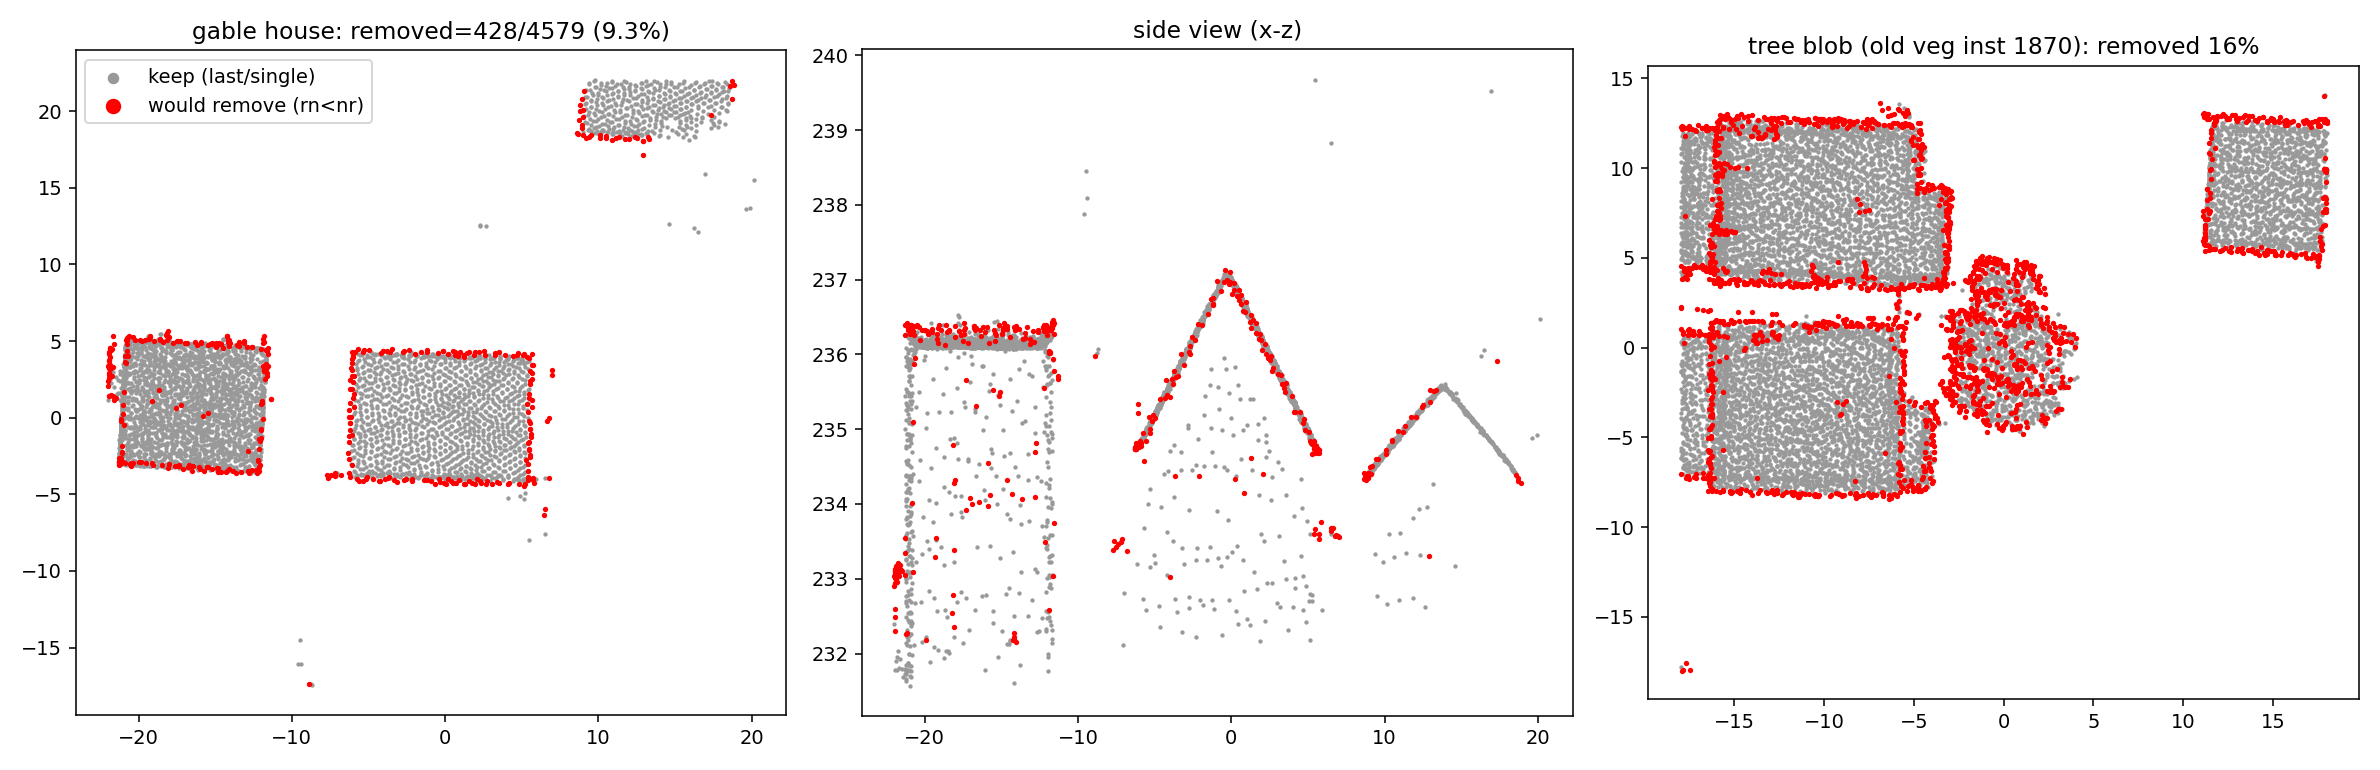
\includegraphics[width=0.98\textwidth]{figs/qa_echo_check.png}
\caption{回波预过滤评估的原始证据（灰 = 保留的单次/末次回波点，红 = 将被删的中间回波点）。
左、中：干净人字顶住宅，428/4{,}579（9.3\%）被删且全部集中在屋檐一圈
（中图侧视可见红点正勾着屋檐边缘）；右：真实树冠污染团，仅 16\% 被删。}
\label{fig:echo}
\end{figure}

\subsection{追溯修正二：6 栋``连体楼''的物理仲裁拆分}

下游轮廓处理阶段发现：少数实例的\textbf{屋顶掩膜}——把该实例的屋顶点投到格子上
得到的黑白图（黑格＝此处有屋顶点）——\textbf{裂成两个互不相连的大块}，
中间隔着被树冠遮挡、没有屋顶点的空白带。
这有两种截然不同的解释，处置完全相反：

\begin{center}
\begin{tabular}{ll}
\toprule
解释 & 正确处置 \\
\midrule
(a) 其实是\textbf{两栋楼}，树把它们桥接了（漏网欠分割） & 拆成两个实例 \\
(b) 是\textbf{一栋大楼}，中段屋顶被树挡住扫不到 & 保持一个实例 \\
\bottomrule
\end{tabular}
\end{center}

肉眼从俯视图上分不出来。我们设计了一个\textbf{物理判据}：

\begin{center}
\fbox{\parbox{0.92\textwidth}{
两栋独立的楼之间是\textbf{露天地面}——激光能从树冠缝隙里穿下去打在地上，
两块之间的``缝走廊''里会出现\textbf{地面（类别 2）点}；而一栋被树遮住中段的大楼，
``缝''的下面是\textbf{实心屋面}，激光穿过树冠碰到的是屋顶，不该出现地面点。
注意证据是\textbf{非对称}的：走廊里\textbf{大量}地面命中是``两栋楼''的强证据；
命中少却不能单独定案（也可能只是树太密、激光下不去）——所以这个判据只用来
\textbf{确认拆分}，不用来单独证明``是一栋''。（还要坦白一点：``类别 2''是第 1 步
模型打的标签，判据的可靠性依赖语义分割对地面的准确率——好在地面是四类里最容易分对的。）
}}
\end{center}

操作：对每个裂成两大块（第二块 $\geq$ 最大块 25\% 面积）的实例，
在两块\textbf{之间}划出走廊——同时距两块都 $\leq3$ 米、又不属于任何一块的格子带
（``同时靠近双方''保证走廊只落在夹缝里）；然后统计：\textbf{分母}＝走廊内全部
1 米格，\textbf{分子}＝其中含类别 2 地面点的格，占比 $\geq 0.35$ 判``两栋楼''。
0.35 是刻意保守的下限——实测中根本没有出现判据附近的灰色案例，分布是干脆的两极：
要么占比极高，要么连两大块都裂不出来。终版审计表（\texttt{split\_verdicts.csv}）里
\textbf{6 个实例命中率 0.96--1.00}（编号 209/217/228/1244/1703/2098，
分别为 1.00/0.96/1.00/1.00/1.00/0.99——几乎每个走廊格都有地面点），
确凿为两栋楼、全部拆分，其中就包括用户在抽查中亲手指认的 228；母实例注销，下游全链重跑。
另有 \textbf{2 个被点名复查的疑似案例}（216/307），检查发现其屋顶掩膜实为一整块
连通区域、根本裂不出两大块（不满足仲裁前提，自然无缝可测），维持单栋判定，证据同样在案。

拆出的 \textbf{12 个新实例编号 2296--2307}。眼尖的读者会发现 2296 与模块 4 的
原编号上限重合：原 2296 号是一个 24.8 m\textsuperscript{2} 的小实例，
已在上一节的树冠追溯中被剔除，编号腾空后被新实例复用——审计表中该编号因此有两行
（旧对象的剔除记录 $+$ 新对象的拆分记录），核对时以判定列区分。

\begin{figure}[H]
\centering
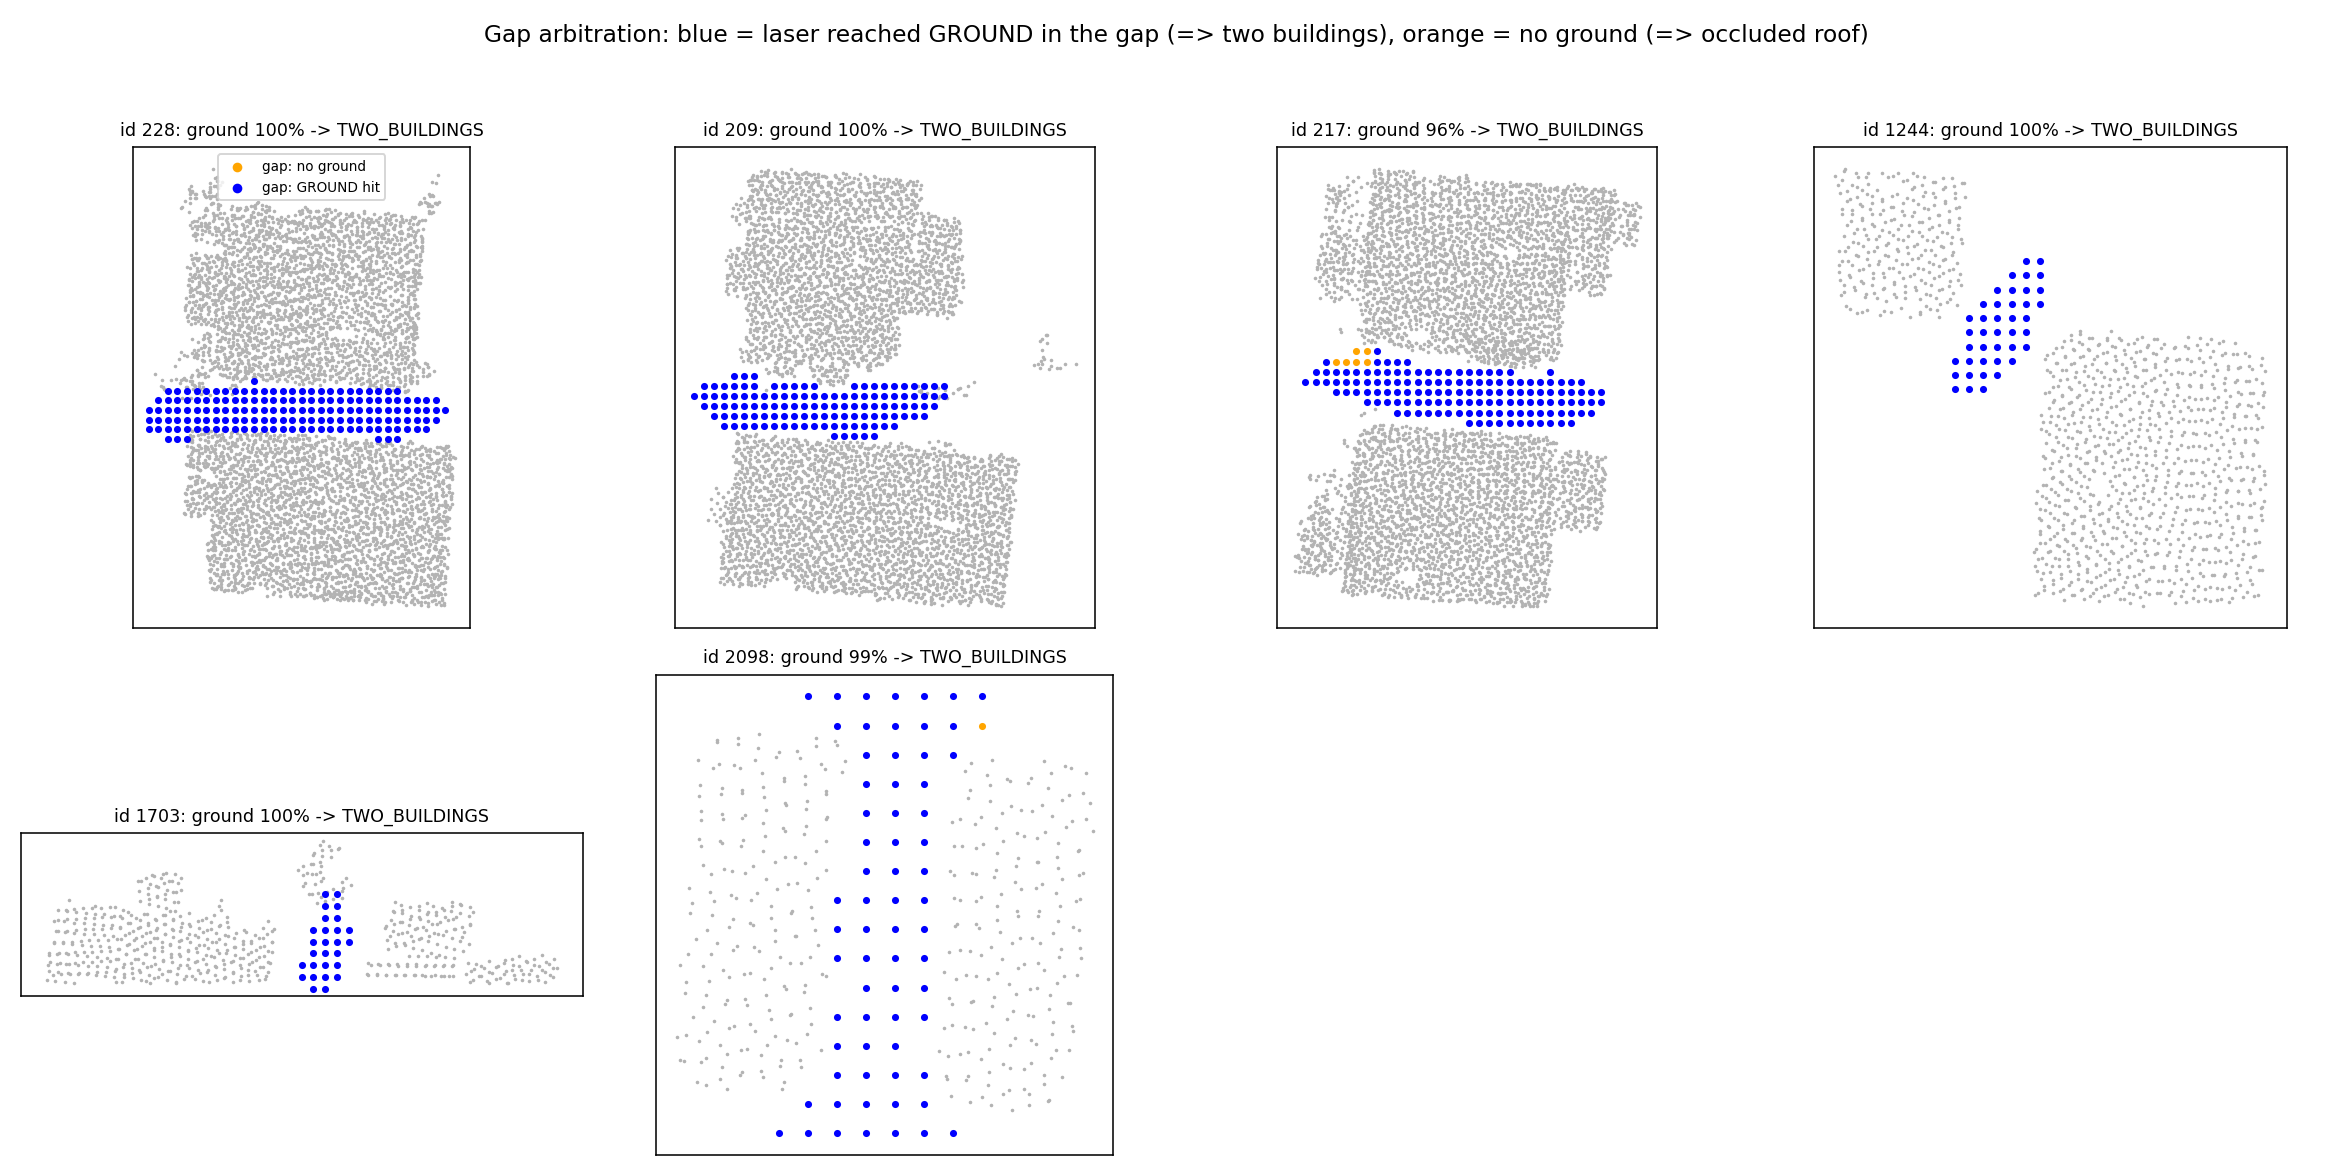
\includegraphics[width=0.95\textwidth]{figs/qa_split_verdicts.png}
\caption{缝内地面命中仲裁：灰 = 屋顶点，蓝 = 走廊内含地面点的格子，橙 = 走廊内无地面点的格子。
六例走廊几乎被蓝点铺满 $\Rightarrow$ 两栋楼（拆分）。两个维持单栋的案例（216/307）
因掩膜连通、无走廊可测，未进入本图。}
\label{fig:split}
\end{figure}

\subsection{最终台账：2{,}296 每一个都有下落}

\begin{numbox}[：逐项对账（数字直接来自审计表 \texttt{instances\_gateA.csv} 的判定列计数）]
\begin{center}
\begin{tabular}{lrl}
\toprule
去向 & 数量 & 说明 \\
\midrule
保留（keep） & 2{,}245 & 判定列为 keep 者——含从未触发规则的多数，也含 A2 复核保留、树冠白名单救回等 \\
细长复核后保留 & 10 & AR$\geq$5 候选中的真实长条建筑（判定列 keep\_reviewed\_ok，模块 5） \\
人工判读剔除 & $-13$ & 桥/匝道/树列/电线，逐个原因码（模块 5） \\
树冠追溯剔除 & $-22$ & 平面性 + 植被上下文 + 目验（本模块） \\
拆分母实例注销 & $-6$ & 缝内地面命中 0.96--1.00（本模块） \\
拆分新生实例 & $+12$ & 编号 2296--2307 \\
\midrule
\textbf{最终干净建筑} & \textbf{2{,}267} & $=2{,}245+10+12$；即 $2{,}296-13-22-6+12$ \\
\bottomrule
\end{tabular}
\end{center}
\end{numbox}

这张表是汇报的``定心丸''：从 2{,}296 到 2{,}267，
每一个消失或新增的编号都有原因码、证据图和存档点云，随时可复查。

\subsection{给 PPT 的建议页序与预答问}

\textbf{建议页序}（每页对应讲义一处，图都是现成的）：
\begin{enumerate}
\item 任务：语义 $\to$ 实例（图~\ref{fig:sem-vs-inst} 重画为 PPT 版）
\item 技术路线一页图：Song \& Jung 骨架 + 分水岭 + 3D BAG 约定（模块 2 总览表）
\item 栅格化与占据规则（图~\ref{fig:raster}）
\item v1 教训：闭运算桥接机理（图~\ref{fig:closing}）+ 检查点复查（图~\ref{fig:checkpoint}）
\item 分水岭拆粘连（图~\ref{fig:erosion-core} + 图~\ref{fig:watershed}；168 拆分战果）
\item Gate A 一页账：HAG（图~\ref{fig:hag}，触发 0 例）；AR 通道 18 候选 $\to$
      8 剔 10 留；A2 通道 25+2 候选 $\to$ 5 剔（图~\ref{fig:solidity}）；合计剔 13
\item 审计总图（图~\ref{fig:gateA}）+ ``规则捞人、人来定罪''原则
\item 追溯修正（上）：树冠 24 候选 $\to$ 22 剔 2 救；回波负结果（图~\ref{fig:echo}）
\item 追溯修正（下）：缝内地面命中仲裁，6 拆、2 不满足前提维持（图~\ref{fig:split}）
\item 台账收官：$2{,}296 \to 2{,}267$ 对账表
\end{enumerate}

\textbf{预答问}（导师高概率提问与推荐答法）：

\begin{itemize}
\item \emph{``为什么不用官方 footprint？''}——研究目标是检验无底图路线的普适性；
      官方 footprint 被有意留作第 9 步的独立评价基准（既当输入又当考卷会让评价失效）。
\item \emph{``为什么不用深度学习做实例分割？''}——无监督路线零训练成本、逐步可审计；
      图聚类新方法（Li 2026）记为候选兜底，本区独栋场景未见必要性。
\item \emph{``0.5 米、$\geq2$ 点这些参数怎么定的？''}——0.5 m 由侧院宽度与点密度共同约束
      （太粗糊缝、太细图斑破碎）；$\geq2$ 点按 30 点/m\textsuperscript{2} 密度下
      0.5 m 格均 7--8 点设定，专杀孤立错点。参数改动都经过检查点复核。
\item \emph{``分水岭会不会把一栋楼错拆成两栋？''}——核有 6 m\textsuperscript{2}
      面积门槛，屋顶毛刺成不了核，从源头压低错拆率；小碎片式的错拆由碎片吸收兜住。
      要诚实承认：``大块对大块''的错拆没有自动纠错（缝内仲裁只负责确认拆分、
      不做反向合并），靠逐楼人工抽查覆盖——本区抽查未发现此类案例。
\item \emph{``删错了怎么办？''}——没有物理删除：全部移仓存档 + 原因码，可整体回滚；
      且删除决定全部经过人工目验，白名单救回 6 例证明流程真实运转。
\item \emph{``树把两栋楼连起来，你怎么发现的？''}——缝内地面命中率：
      激光穿过树冠缝隙会在露天缝里打出地面点，实心屋面下则不会。
      6 例命中 0.96--1.00、无灰色案例，物理判据干脆。
\end{itemize}

\begin{plainbox}[：模块 6 小结（也是全讲义收尾）]
步骤 2--3 的完整故事：863 万建筑点 $\to$ 栅格化 + 连通域（不做闭运算）
$\to$ 分水岭拆 168 处粘连 $\to$ 2{,}296 候选 $\to$ Gate A 规则捞人、人工定罪（$-13$）
$\to$ 下游证据追溯修正（$-22$ 树冠、6 拆 12）$\to$ \textbf{2{,}267 栋干净建筑}，
每一步有论文依据、每一个决定有原因码、每一批数字可对账。
\end{plainbox}

\newpage
\section*{附录 · 术语速查表}
\addcontentsline{toc}{section}{附录 · 术语速查表}
\markboth{附录 · 术语速查表}{附录 · 术语速查表}

正文对每个术语都有解释（少数术语首次露面时只作预告、到对应模块才详细展开）。
此表按各术语\textbf{主要讲解位置}的先后排列，供汇报前快速复习。

\begin{center}
\small
\begin{tabular}{p{3.4cm}p{11.2cm}}
\toprule
术语 & 一句话解释 \\
\midrule
\multicolumn{2}{l}{\emph{—— 模块 1 ——}} \\
LiDAR（激光雷达） & 飞机向地面发激光、按反射时间测距的技术，产出即点云 \\
点云 & LiDAR 测得的大量三维坐标点的集合，像``由点组成的三维照片'' \\
高程 & 相对统一高度基准面的高度（不是``离地面多高''） \\
ftUS & 美制测量英尺，$\approx0.3048$ 米；美国官方测绘数据的惯例单位 \\
瓦片（tile） & 大区域数据切成的分块文件，本项目共 19 块 \\
LAZ & 点云的压缩文件格式（LAS 是标准点云格式，LAZ 是其压缩版） \\
语义分割 & 给每个点贴类别标签（地面 2/植被 5/建筑 6/其他 1），回答``是什么'' \\
实例分割 / 单体化 & 给每个建筑点一个楼编号（instance\_id），回答``是哪一栋'' \\
欠分割 / 过分割 & 该分开的没分开（楼粘成一条）/ 不该分的被拆碎（一栋变几块） \\
Gate A & 实例级噪声闸门：规则捞候选 + 人工定罪 + 原因码存档（模块 5--6 详述） \\
\multicolumn{2}{l}{\emph{—— 模块 2 ——}} \\
CloudCompare & 免费点云查看软件，本项目每步人工抽查的工具 \\
footprint（建筑底图） & 现成的每栋楼平面轮廓多边形；本项目不用作输入，留作最终评价基准 \\
\multicolumn{2}{l}{\emph{—— 模块 3 ——}} \\
栅格化 & 把连续空间切成规则方格并统计每格内容（本项目格边长 0.5 m） \\
占据格 & 落入 $\geq2$ 个建筑点的格子；全部占据格构成黑白``占据图'' \\
连通域 & 黑白图上互相挨着的黑格归成的``块''；8-连通 = 斜角也算挨着 \\
形态学操作 & 对黑白图的修形操作家族（膨胀、腐蚀、闭运算等） \\
膨胀 / 腐蚀 & 黑色区域向外长一圈 / 向内削一圈（厚度由结构元定） \\
结构元 & 规定每次扩/削多远的小模板（如 $3\times3$ = 周围一圈） \\
闭运算 & 先膨胀再腐蚀；会把楼间窄缝焊死——v1 的事故根源，v2 已弃用 \\
填洞（fill holes） & 只填被完全包围的内部空洞、不碰向外开口的缝——v2 的补洞方式 \\
\multicolumn{2}{l}{\emph{—— 模块 4 ——}} \\
核（core） & 块被腐蚀 1.5 m 后剩下的 $\geq6$ m\textsuperscript{2} 主体；个数用于估计栋数，并充当分水岭水源 \\
分水岭算法 & 把图当地形灌水、两片水相遇处筑坝作为分割边界的经典算法 \\
marker & 分水岭的指定水源；本项目用``核''充当，压住过分割 \\
$z_{\max}$ 高度图 & 每格记录格内最高点高程；取负后作为分水岭的``地形'' \\
中位数 / 百分位 & 排队取正中间的值 / 排队取指定百分比位置的值（$P_5$ = 从低往高 5\% 处） \\
碎片吸收 & $<20$ m\textsuperscript{2} 的碎片并入\textbf{平面距离 3 m 内、面积 $\geq50$ m\textsuperscript{2}、中位高程差 $\leq3$ m} 的最近``锚''实例（锚 = 吸收方；只许小并大） \\
孤儿点回挂 & 因所在格不足 2 点而暂未分块的点，回挂到 1.5 m 内最近实例格 \\
防撞色 & 每个实例随机分配且保证与邻居不同的显示颜色，避免``相邻同色''误读 \\
\multicolumn{2}{l}{\emph{—— 模块 5 ——}} \\
DTM & 数字地形模型：一张``每个位置的地面高程''图，由类别 2 地面点建成 \\
HAG（离地高度） & 实例中位高程 $z_{50}$ 减周围 4 m 环带内 DTM 的 $P_5$（环带只取有实测地面点的格，不足 20 个才用填补值） \\
长宽比 AR & 实例平面形状``最长伸展 / 最宽伸展''之比（求点分布伸展最大与最小的方向再作比），细长体侦测用 \\
凸包 & ``橡皮筋箍住形状''得到的最小凸多边形 \\
充实度 solidity & 实例面积 ÷ 凸包面积；本区实测折带 0.4--0.6、建筑主体 $>0.75$（候选门槛 0.72，终裁靠人工） \\
距离变换 EDT & 算形状内每点到边界的距离；最大值 $\times2$ = 形状``最宽处宽度'' \\
伸长指标 elong & 面积 $\div$ 最宽处宽度$^2$；同面积下越``带状''越大（候选门槛 3.5），抓方正桥板的补网 \\
原因码 & 审计表中每个剔除/拆分决定的机器可读理由（如 \texttt{reject\_reviewed\_powerline}） \\
移仓存档 & 被剔除的点不删除，单独存成文件（\texttt{noise\_removed.laz} 等）可回看回滚 \\
\multicolumn{2}{l}{\emph{—— 模块 6 ——}} \\
回波（return） & 一束激光的多次反射；``中间回波''= 多次回波中\textbf{非最后一次}的回波（首次也可能是，如``第 1 次/共 2 次''），树冠的典型特征 \\
选择偏差 & 被模型错标的子集与总体特征分布不同——``植被点 94.8\% 中间回波''不适用于``被错标的那部分树点'' \\
追溯修正（retro） & 下游步骤的新证据回传、推翻 Gate A 早先判决的机制 \\
缝内地面命中 & 判连体楼的物理判据：两块屋顶间走廊内\textbf{含类别 2 地面点的 1 m 格占比} $\geq0.35$ 判两栋（激光穿过树冠缝隙打到露天地面；实心屋面下无地面回波） \\
\bottomrule
\end{tabular}
\end{center}


\end{document}
